\documentclass[10pt]{article}
\usepackage[T1]{fontenc}
\usepackage{amsmath,amssymb,amsthm}
\usepackage{mathtools}
\usepackage[shortlabels]{enumitem}
\usepackage[english]{babel}
\usepackage[utf8]{inputenc}
\usepackage{fancyhdr}
\usepackage{bold-extra}
\usepackage{color}   
\usepackage{tocloft}
\usepackage{graphicx}
\usepackage{lipsum}
\usepackage{wrapfig}
\usepackage{cutwin}
\usepackage{hyperref}
\usepackage{lastpage}
\usepackage{multicol}
\usepackage{tikz}
\usepackage{xcolor}
\usepackage{microtype}
\usetikzlibrary{positioning, fit, calc}
\usepackage[framemethod=TikZ]{mdframed}

% some useful math commands
\newcommand{\eps}{\varepsilon}
\newcommand{\R}{\mathbb{R}}
\newcommand{\C}{\mathbb{C}}
\newcommand{\N}{\mathbb{N}}
\newcommand{\Z}{\mathbb{Z}}
\newcommand{\Q}{\mathbb{Q}}
\newcommand{\K}{\mathbb{K}}
\newcommand{\F}{\mathbb{F}}
\newcommand{\T}{\mathbb{T}}

\newcommand{\Poly}{\mathbf{P}}
\newcommand{\NP}{\mathbf{NP}}

\numberwithin{equation}{section}

\newcommand{\dd}{\,\mathrm{d}}
\newcommand{\ddz}{\frac{\rm d}{{\rm d}z}}
\newcommand{\pv}{\text{p.v.}}

\renewcommand{\Re}{{\rm Re}}

\DeclareMathOperator{\GL}{GL}
\DeclareMathOperator{\id}{id}
\DeclareMathOperator{\Arg}{Arg}
\DeclareMathOperator{\Log}{Log}
\DeclareMathOperator{\PV}{PV}
\DeclareMathOperator{\sech}{sech}
\DeclareMathOperator{\csch}{csch}
\DeclareMathOperator{\Res}{Res}
\DeclareMathOperator{\Li}{Li}
\DeclareMathOperator{\QR}{QR}
\DeclareMathOperator{\NR}{NR}
\DeclareMathOperator{\lcm}{lcm}
\DeclareMathOperator{\divergence}{div}
\DeclareMathOperator*{\esssup}{ess\,sup}
\DeclareMathOperator{\Span}{span}
\DeclareMathOperator{\Pol}{Pol}
\DeclareMathOperator*{\argmin}{arg\,min}
\DeclareMathOperator*{\argmax}{arg\,max}

\DeclarePairedDelimiter\ceil{\lceil}{\rceil}
\DeclarePairedDelimiter\floor{\lfloor}{\rfloor}

\newcommand{\suchthat}{\;\ifnum\currentgrouptype=16 \;\middle|\;\else\mid\fi\;}

% title formatting
\newcommand{\newtitle}[4]{
  \begin{center}
	\huge{\textbf{\textsc{#1 Course Notes}}}
    
	\large{\sc #2}
    
	{\sc #3 \textbullet\, #4 \textbullet\, University of Waterloo}
	\normalsize\vspace{1cm}\hrule
  \end{center}
}

\newcounter{theo}[section]\setcounter{theo}{0}
\renewcommand{\thetheo}{\arabic{section}.\arabic{theo}}
\newenvironment{theo}[2][]{%
\refstepcounter{theo}%
\ifstrempty{#1}%
{\mdfsetup{%
frametitle={%
\tikz[baseline=(current bounding box.east),outer sep=0pt]
\node[anchor=east,rectangle,fill=blue!20]
{\strut {\sc Theorem~\thetheo}};}}
}%
{\mdfsetup{%
frametitle={%
\tikz[baseline=(current bounding box.east),outer sep=0pt]
\node[anchor=east,rectangle,fill=blue!20]
{\strut {\sc Theorem~\thetheo:~#1}};}}%
}%
\mdfsetup{innertopmargin=10pt,linecolor=blue!20,%
linewidth=2pt,topline=true,%
frametitleaboveskip=\dimexpr-\ht\strutbox\relax
}
\begin{mdframed}[nobreak=false]\relax%
\label{#2}}{\end{mdframed}}

%%%%%%%%%%%%%%%%%%%%%%%%%%%%%%
%Definition
\newenvironment{defn}[2][]{%
\refstepcounter{theo}%
\ifstrempty{#1}%
{\mdfsetup{%
frametitle={%
\tikz[baseline=(current bounding box.east),outer sep=0pt]
\node[anchor=east,rectangle,fill=yellow!20]
{\strut {\sc Definition~\thetheo}};}}
}%
{\mdfsetup{%
frametitle={%
\tikz[baseline=(current bounding box.east),outer sep=0pt]
\node[anchor=east,rectangle,fill=yellow!20]
{\strut {\sc Definition~\thetheo:~#1}};}}%
}%
\mdfsetup{innertopmargin=10pt,linecolor=yellow!20,%
linewidth=2pt,topline=true,%
frametitleaboveskip=\dimexpr-\ht\strutbox\relax
}
\begin{mdframed}[nobreak=true]\relax%
\label{#2}}{\end{mdframed}}

%%%%%%%%%%%%%%%%%%%%%%%%%%%%%%
%Example
\newenvironment{exmp}[2][]{%
\refstepcounter{theo}%
\ifstrempty{#1}%
{\mdfsetup{%
frametitle={%
\tikz[baseline=(current bounding box.east),outer sep=0pt]
\node[anchor=east,rectangle,fill=cyan!20]
{\strut {\sc Example~\thetheo}};}}
}%
{\mdfsetup{%
frametitle={%
\tikz[baseline=(current bounding box.east),outer sep=0pt]
\node[anchor=east,rectangle,fill=cyan!20]
{\strut {\sc Example~\thetheo:~#1}};}}%
}%
\mdfsetup{innertopmargin=10pt,linecolor=cyan!20,%
linewidth=2pt,topline=true,%
frametitleaboveskip=\dimexpr-\ht\strutbox\relax
}
\begin{mdframed}[nobreak=false]\relax%
\label{#2}}{\end{mdframed}}

%%%%%%%%%%%%%%%%%%%%%%%%%%%%%%
%Corollary
\newenvironment{cor}[2][]{%
\refstepcounter{theo}%
\ifstrempty{#1}%
{\mdfsetup{%
frametitle={%
\tikz[baseline=(current bounding box.east),outer sep=0pt]
\node[anchor=east,rectangle,fill=lime!20]
{\strut {\sc Corollary~\thetheo}};}}
}%
{\mdfsetup{%
frametitle={%
\tikz[baseline=(current bounding box.east),outer sep=0pt]
\node[anchor=east,rectangle,fill=lime!20]
{\strut {\sc Corollary~\thetheo:~#1}};}}%
}%
\mdfsetup{innertopmargin=10pt,linecolor=lime!20,%
linewidth=2pt,topline=true,%
frametitleaboveskip=\dimexpr-\ht\strutbox\relax
}
\begin{mdframed}[nobreak=true]\relax%
\label{#2}}{\end{mdframed}}

%%%%%%%%%%%%%%%%%%%%%%%%%%%%%%
%Remark
\newenvironment{remark}[2][]{%
\refstepcounter{theo}%
\ifstrempty{#1}%
{\mdfsetup{%
frametitle={%
\tikz[baseline=(current bounding box.east),outer sep=0pt]
\node[anchor=east,rectangle,fill=orange!20]
{\strut {\sc Remark~\thetheo}};}}
}%
{\mdfsetup{%
frametitle={%
\tikz[baseline=(current bounding box.east),outer sep=0pt]
\node[anchor=east,rectangle,fill=orange!20]
{\strut {\sc Remark~\thetheo:~#1}};}}%
}%
\mdfsetup{innertopmargin=10pt,linecolor=orange!20,%
linewidth=2pt,topline=true,%
frametitleaboveskip=\dimexpr-\ht\strutbox\relax
}
\begin{mdframed}[nobreak=true]\relax%
\label{#2}}{\end{mdframed}}

%%%%%%%%%%%%%%%%%%%%%%%%%%%%%%
%Exercise
\newenvironment{exercise}[2][]{%
\refstepcounter{theo}%
\ifstrempty{#1}%
{\mdfsetup{%
frametitle={%
\tikz[baseline=(current bounding box.east),outer sep=0pt]
\node[anchor=east,rectangle,fill=pink!20]
{\strut {\sc Exercise~\thetheo}};}}
}%
{\mdfsetup{%
frametitle={%
\tikz[baseline=(current bounding box.east),outer sep=0pt]
\node[anchor=east,rectangle,fill=pink!20]
{\strut {\sc Exercise~\thetheo:~#1}};}}%
}%
\mdfsetup{innertopmargin=10pt,linecolor=pink!20,%
linewidth=2pt,topline=true,%
frametitleaboveskip=\dimexpr-\ht\strutbox\relax
}
\begin{mdframed}[nobreak=true]\relax%
\label{#2}}{\end{mdframed}}

%%%%%%%%%%%%%%%%%%%%%%%%%%%%%%
%Lemma
\newenvironment{lemma}[2][]{%
\refstepcounter{theo}%
\ifstrempty{#1}%
{\mdfsetup{%
frametitle={%
\tikz[baseline=(current bounding box.east),outer sep=0pt]
\node[anchor=east,rectangle,fill=green!20]
{\strut {\sc Lemma~\thetheo}};}}
}%
{\mdfsetup{%
frametitle={%
\tikz[baseline=(current bounding box.east),outer sep=0pt]
\node[anchor=east,rectangle,fill=green!20]
{\strut {\sc Lemma~\thetheo:~#1}};}}%
}%
\mdfsetup{innertopmargin=10pt,linecolor=green!20,%
linewidth=2pt,topline=true,%
frametitleaboveskip=\dimexpr-\ht\strutbox\relax
}
\begin{mdframed}[nobreak=true]\relax%
\label{#2}}{\end{mdframed}}

%%%%%%%%%%%%%%%%%%%%%%%%%%%%%%
%Proposition
\newenvironment{prop}[2][]{%
\refstepcounter{theo}%
\ifstrempty{#1}%
{\mdfsetup{%
frametitle={%
\tikz[baseline=(current bounding box.east),outer sep=0pt]
\node[anchor=east,rectangle,fill=purple!20]
{\strut {\sc Proposition~\thetheo}};}}
}%
{\mdfsetup{%
frametitle={%
\tikz[baseline=(current bounding box.east),outer sep=0pt]
\node[anchor=east,rectangle,fill=purple!20]
{\strut {\sc Proposition~\thetheo:~#1}};}}%
}%
\mdfsetup{innertopmargin=10pt,linecolor=purple!20,%
linewidth=2pt,topline=true,%
frametitleaboveskip=\dimexpr-\ht\strutbox\relax
}
\begin{mdframed}[nobreak=true]\relax%
\label{#2}}{\end{mdframed}}

%%%%%%%%%%%%%%%%%%%%%%%%%%%%%%
%Fact
\newenvironment{fact}[2][]{%
\refstepcounter{theo}%
\ifstrempty{#1}%
{\mdfsetup{%
frametitle={%
\tikz[baseline=(current bounding box.east),outer sep=0pt]
\node[anchor=east,rectangle,fill=gray!20]
{\strut {\sc Fact~\thetheo}};}}
}%
{\mdfsetup{%
frametitle={%
\tikz[baseline=(current bounding box.east),outer sep=0pt]
\node[anchor=east,rectangle,fill=gray!20]
{\strut {\sc Fact~\thetheo:~#1}};}}%
}%
\mdfsetup{innertopmargin=10pt,linecolor=gray!20,%
linewidth=2pt,topline=true,%
frametitleaboveskip=\dimexpr-\ht\strutbox\relax
}
\begin{mdframed}[nobreak=true]\relax%
\label{#2}}{\end{mdframed}}

% new proof environment
\newenvironment{pf}[1][\proofname]
  {\par\noindent\normalfont\textbf{Proof of #1.}\par\nopagebreak%
  \begin{mdframed}[
     linewidth=1pt,
     linecolor=black,
     bottomline=false,topline=false,rightline=false,
     innerrightmargin=0pt,innertopmargin=0pt,innerbottommargin=0pt,
     innerleftmargin=1em,% Distance between vertical rule & proof content
     skipabove=0.75\baselineskip
   ]}
  {\end{mdframed}}

% 1-inch margins
\topmargin 0pt
\advance \topmargin by -\headheight
\advance \topmargin by -\headsep
\textheight 8.9in
\oddsidemargin 0pt
\evensidemargin \oddsidemargin
\marginparwidth 0.5in
\textwidth 6.5in

\parindent 0in
\parskip 1.5ex

\setlist[itemize]{topsep=0pt}
\setlist[enumerate]{topsep=0pt}

\newcommand{\pushright}[1]{\ifmeasuring@#1\else\omit\hfill$\displaystyle#1$\fi\ignorespaces}

% hyperlinks
\hypersetup{
  colorlinks=true, 
  linktoc=all,     % table of contents is clickable  
  allcolors=red    % all hyperlink colours
}

% table of contents
\addto\captionsenglish{
  \renewcommand{\contentsname}%
    {Table of Contents}%
}
\renewcommand{\cftsecfont}{\normalfont}
\renewcommand{\cftsecpagefont}{\normalfont}
\cftsetindents{section}{0em}{2em}

\fancypagestyle{plain}{%
\fancyhf{} % clear all header and footer fields
\lhead{CO 353: Winter 2023}
\fancyhead[R]{Table of Contents}
%\headrule
\fancyfoot[R]{{\small Page \thepage\ of \pageref*{LastPage}}}
}

% headers and footers
\pagestyle{fancy}
\renewcommand{\sectionmark}[1]{\markboth{#1}{#1}}
\lhead{CO 353: Winter 2023}
\cfoot{}
\setlength\headheight{14pt}

%\setcounter{section}{-1}

\begin{document}

\pagestyle{fancy}
\newtitle{CO 353}{Computational Discrete Optimization}{Kanstantsin Pashkovich}{Winter 2023}
\rhead{Table of Contents}
\rfoot{{\small Page \thepage\ of \pageref*{LastPage}}}

\tableofcontents
\vspace{1cm}\hrule
\fancyhead[R]{\nouppercase\rightmark}
\newpage 
\fancyhead[R]{Section \thesection: \nouppercase\leftmark}

\section{Shortest Paths}\label{sec:1}

\subsection{Preliminaries on Graphs}\label{subsec:1.1}
An {\bf (undirected) graph} $G$ is a pair $(V, E)$, where $E$ is a set of 
unordered pairs of elements in $V$. The elements of $V$ are called {\bf vertices}
or {\bf nodes}; the elements of $E$ are called {\bf edges}. 

Let $u, v \in V$ and let $e = uv \in E$ be an edge. 
\begin{itemize}
    \item We say that $e$ is {\bf incident} to $u$ and $v$. 
    \item The vertices $u$ and $v$ are said to be {\bf adjacent}.
    \item We call $u$ and $v$ the {\bf endpoints} of $e$. 
\end{itemize}
By default, we assume that there are no parallel edges (i.e. two
edges $e = uv$ and $e' = u'v'$ in $E$ with $\{u, v\} = \{u', v'\}$) 
and no loops (i.e. an edge $e = uv \in E$ with $u = v$).

For distinct $u, v \in V$, a {\bf $u, v$-path} is a sequence of vertices 
$w_1, \dots, w_k$ such that $w_1 = u$, $w_k = v$, and $w_i w_{i+1} \in E$ 
for all $i = 1, \dots, k-1$.  

For example, consider the following graph $G = (V, E)$ with 
vertices $V = \{v_1, v_2, v_3, v_4\}$ and edges $E = \{v_1v_2, v_1v_4, v_2v_3, 
v_2v_4, v_3v_4\}$. 

\begin{center}
    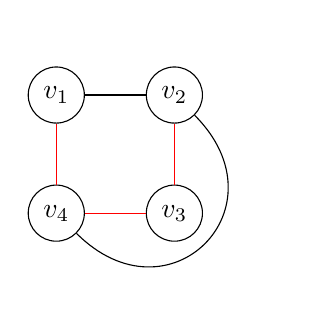
\begin{tikzpicture}[node distance={15mm}, main/.style = {draw, circle}] 
        \node[main] (1) {$v_1$}; 
        \node[main] (2) [right of=1] {$v_2$};
        \node[main] (3) [below of=2] {$v_3$}; 
        \node[main] (4) [left of=3] {$v_4$};

        \draw (1) -- (2);
        \draw [draw=red] (1) -- (4);
        \draw [draw=red] (2) -- (3);
        \draw (2) to [out=315, in=315, looseness=2] (4);
        \draw [draw=red] (3) -- (4);
    \end{tikzpicture} 
\end{center}
\vspace{-0.5cm}

The lines in red form a $v_1, v_2$-path, namely $v_1, v_4, v_3, v_2$. 
Another $v_1, v_2$-path can be obtained by simply traversing the edge $v_1v_2$. 

A {\bf cycle} in $G$ is a sequence of vertices $w_1, \dots, w_{k+1}$ 
such that $w_i w_{i+1} \in E$ for all $i = 1, \dots, k$, the vertices 
$w_1, \dots, w_k$ are all distinct, and $w_1 = w_{k+1}$.

Finally, a graph $G$ is {\bf connected} if for any pair of distinct vertices 
$u, v \in V$, there exists a $u, v$-path in $G$. 

\subsection{Shortest Paths Problem}\label{subsec:1.2}
Given a \emph{directed} graph $G = (V, E)$ with edge lengths $\ell_e \geq 0$
for each $e \in E$ and a distinguished start vertex $s \in V$, we wish 
to find shortest paths from $s$ to every other vertex in $V$. Note that 
when we work with directed graphs, we will denote the directed edges 
with $(v_1, v_2)$ as opposed to $v_1 v_2$ in the case of undirected graphs, where 
the order of the vertices did not matter. 

The {\bf length} of a path $P$ given by the sequence $w_1, \dots, w_k$ 
is given by 
\[ \ell(P) := \sum_{i=1}^{k-1} \ell_{(w_i, w_{i+1})} = \sum_{e\in P} \ell_e, \] 
where the second sum makes sense because there are no parallel edges. 
Then the {\bf shortest-path distance} from $s$ to a vertex $u \in V$ is 
defined to be
\[ d(u) := \min_{\text{$s,u$-paths $P$}} \ell(P). \] 
For example, we can consider the following instance of an undirected graph 
with given edge lengths and starting vertex $s = v_1$. 

\begin{center}
    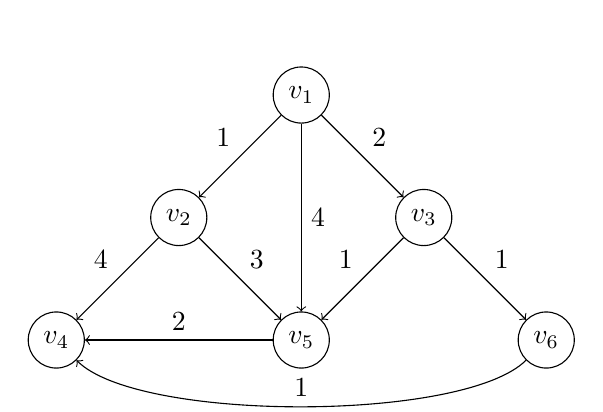
\begin{tikzpicture}[node distance={22mm}, main/.style = {draw, circle}] 
        \node[main] (1) {$v_1$}; 
        \node[main] (2) [below left of=1] {$v_2$};
        \node[main] (3) [below right of=1] {$v_3$}; 
        \node[main] (4) [below left of=2] {$v_4$};
        \node[main] (5) [below left of=3] {$v_5$};
        \node[main] (6) [below right of=3] {$v_6$};

        \draw[->] (1) -- node[midway, above left] {1} (2);
        \draw[->] (1) -- node[midway, above right] {2} (3);
        \draw[->] (1) -- node[midway, right] {4} (5);
        \draw[->] (2) -- node[midway, above left] {4} (4);
        \draw[->] (2) -- node[midway, above right] {3} (5);
        \draw[->] (3) -- node[midway, above left] {1} (5);
        \draw[->] (3) -- node[midway, above right] {1} (6);
        \draw[->] (5) -- node[midway, above] {2} (4);
        \draw[->] (6) to [out=225, in=315, looseness=0.5] node[midway, above] {1} (4);
    \end{tikzpicture} 
\end{center}
\vspace{-0.5cm}
In this case, we have $d(v_2) = 1$, since the only possible path from 
$v_1$ to $v_2$ is by taking the edge $(v_1, v_2)$. There are multiple
paths from $v_1$ to $v_5$; the shortest one is $v_1, v_3, v_5$ giving 
$d(v_5) = 3$. 

Note that we always set $d(s) = 0$. We now make some observations: 
\begin{enumerate}[(i)]
    \item If $(u, v) \in E$, then $d(v) \leq d(u) + \ell_{(u,v)}$, since 
    such an $s, v$-path is always an option.
    \item For every $v \in V$ distinct from $s$, there exists $w \in V$ 
    such that $d(v) = d(w) + \ell_{(w, v)}$ and $(w, v) \in E$. This can 
    be seen by chopping off the last edge from a shortest path from $s$ to $v$.
\end{enumerate}

\subsection{Dijkstra's Algorithm}\label{subsec:1.3}
In 1959, Dijkstra came up with the following algorithm to solve the 
shortest paths problem. The main idea is to maintain a set $A \subseteq V$ 
of ``explored'' nodes; that is, a set of nodes for which we already know the 
shortest-path distances. We'll also maintain labels $d'(v)$ for $v \in 
V \setminus A$ with upper bounds on the shortest-path distances from $s$. 

\begin{mdframed}[
    linewidth=1pt,
    linecolor=black,
    bottomline=false,topline=false,rightline=false,
    innerrightmargin=0pt,innertopmargin=0pt,innerbottommargin=0pt,
    innerleftmargin=1em,% Distance between vertical rule & proof content
    skipabove=0.75\baselineskip
]
{\bf Input.} A directed graph $G = (V, E)$, edge lengths $\ell_e \geq 0$ for 
all $e \in E$, and a start vertex $v \in V$. 

{\bf Output.} For all $v \in V$, the length $d(v)$ for the shortest-path from 
$s$ to $v$.
\begin{enumerate}[leftmargin=1.75cm, label={Step \arabic*.}]
    \item {\bf (Initialization.)} Set $A \gets \{s\}$, $d(s) \gets 0$, and $d'(v) \gets \infty$ 
    for all $v \in V \setminus A$.

    \item While $A \neq V$:
    \begin{enumerate}[label={Step 2.\arabic*.}]
        \item {\bf (Push down the upper bounds.)} For each $v \in V \setminus A$, compute 
        \[ d'(v) \gets \min\left\{ d'(v), \min_{\substack{u\in A \\ (u, v) \in E}} 
        \{ d(u) + \ell_{(u, v)} \} \right\}. \] 
        \item {\bf (Add a new vertex.)} Set $w \gets \argmin_{v \in V \setminus A} d'(v)$, 
        $A \gets A \cup \{w\}$, and $d(w) \gets d'(w)$. 
    \end{enumerate}
\end{enumerate}
\end{mdframed}\vspace{-0.25cm}

Suppose that for each vertex $w \in V$, we keep track of the node $u$ 
determining its upper bound $d'(w)$. That is, the node $u$ is such that 
$(u, w) \in E$ and $d'(w) = d(u) + \ell_{(u, w)}$. Then at the end of the 
algorithm, a shortest path from $s$ to $w$ can be obtained as a shortest path 
from $s$ to $u$ adjoined with the edge $(u, w) \in E$. Moreover, these edges 
selected by Dijkstra's algorithm form an arborescence, which is a nice graph 
structure that we'll discuss more later. 

Next, let's prove the correctness of Dijkstra's algorithm. In particular, 
we need to show that for every $v \in V$, the distance from $s$ to $v$ 
is computed correctly. We'll assume that the graph is connected; that is, 
for every $v \in V$, there is an $s, v$-path in $G$. (Note that the 
algorithm won't terminate otherwise, but it can be adjusted to deal 
with this.)

\begin{pf}[correctness of Dijkstra's algorithm]
    We proceed by induction on $|A|$, and show that at each point in time, 
    $d(v)$ is computed correctly for all $v \in A$. The case where $|A| = 1$ 
    is clear because at the start of the algorithm, we initialize $A = \{s\}$ 
    with $d(s) = 0$, which is correct. 

    Assume that $d(v)$ is computed correctly for every $v \in A$ when 
    that $|A| = k$. Suppose that we are adding a new vertex $w$ to $A$ 
    in Step 2.2 of the algorithm. Consider the vertex $u \in A$ such that 
    $(u, w) \in E$ and 
    \[ d'(w) = d(u) + \ell_{(u, w)}. \] 
    Specifically, this is the vertex $u$ determining the upper bound 
    $d'(w)$ which we discussed in the paragraph following the description 
    of the algorithm. 

    For the sake of contradiction, assume that the distance from $s$ to $w$ 
    is not $d'(w)$. Let $P_u$ be a shortest path from $s$ to $u$, and 
    let $P'$ be a shortest path from $s$ to $w$. Then by our 
    assumption, we know that 
    \[ \ell(P') < \ell(P_u) + \ell_{(u, w)} = d'(w). \] 
    Now, let $x, y \in V$ be such that $(x, y) \in E$ lies on the shortest 
    path $P'$ from $s$ to $w$, with $x \in A$ and $y \in V \setminus A$. 
    (This exists because at some point, the path must exit $A$ to get 
    from $s$ to $w$.) Then we obtain 
    \[ d'(y) \leq d(x) + \ell_{(x,y)} \leq \ell(P') < \ell(P_u) 
    + \ell_{(u, w)} = d'(w), \] 
    where the first inequality is because of how $d'(y)$ is computed in 
    Step 2.1, and the second inequality is because the shortest path 
    from $x$ to $y$ adjoined with the edge $(x, y)$ is part of the path $P'$, 
    noting that $\ell_e \geq 0$ for all $e \in E$. But this contradicts 
    our choice of $w = \argmin_{v\in V \setminus A} \{d'(v)\}$ in Step 2.2 
    since $y \in V \setminus A$ but $d'(y) < d'(w)$. \qed
\end{pf}\vspace{-0.25cm}

The {\bf running time} of an algorithm is the number of elementary operations 
that the algorithm performs as a function of the input size. The {\bf input 
size} is the number of bits needed to specify the input. 
\begin{itemize}
    \item For example, in order to specify an integer $n \geq 0$ in binary, 
    we require about $\log_2(n)$ bits. 
    \item To specify a graph $G = (V, E)$ with integral edge lengths 
    $\ell_e \geq 0$ for each $e \in E$, we require approximately 
    $|V| + |E| + \sum_{e\in E} \log_2(\ell_e)$ bits. Note that we can 
    specify an edge with two pointers to the endpoints.
\end{itemize} 
We will need big-$O$ notation to describe running time, because we are 
interested in the asymptotic behaviour of algorithms. For two functions
$f : \R^+ \to \R^+$ and $g : \R^+ \to \R^+$, we say that $f(n) = 
O(g(n))$ if there exist constants $n_0 \in \N$ and $c \geq 0$ such that 
$f(n) \leq c \cdot g(n)$ for all $n \geq n_0$. For example, we have 
$2n^2 + 1 = O(n^2)$ and $\log(n) = O(n)$. An algorithm is then considered 
{\bf efficient} if its running time is bounded above by a polynomial function 
of the input size. 

Let's consider the running time of Dijkstra's algorithm by looking 
at a naive implementation. For ease of notation, we will write 
$|V| = n$ and $|E| = m$. Note that $G = (V, E)$ is connected, 
so $n-1 \leq m \leq n^2$.
\begin{itemize}
    \item Step 1 can be performed using $O(n)$ operations since we are only
    assigning values for each vertex. 
    \item In Step 2, there are at most $n$ iterations. 
    \begin{itemize}
        \item Step 2.1 can be performed using $O(m)$ operations because 
        each edge will participate in at most two comparisons throughout the 
        entire iteration. 
        \item Step 2.2 takes $O(n)$ operations in order to determine the 
        vertex of minimum upper bound. 
    \end{itemize}
\end{itemize}
Therefore, the running time of the naive implementation is 
$O(n + mn + n^2) = O(mn)$, which is polynomial in the input size.  

We note that there are better implementations of Dijkstra's algorithm 
than the naive one that we have just stated. For Step 2.1, we can 
use $m$ \textsc{Decrease-Key} calls and for Step 2.2, we can use 
$n$ \textsc{Extract-Min} calls. In particular, by using Fibonacci heaps, 
\textsc{Decrease-Key} has running time $O(1)$ and \textsc{Extract-Min} 
has running time $O(\log n)$, which brings the total running time down to 
$O(m + n\log n)$.\newpage
\section{Minimum Spanning Trees}\label{sec:2}

\subsection{Trees}\label{subsec:2.1}
A {\bf tree} is a connected acyclic graph; that is, a connected graph 
containing no cycles. 
\begin{center}
    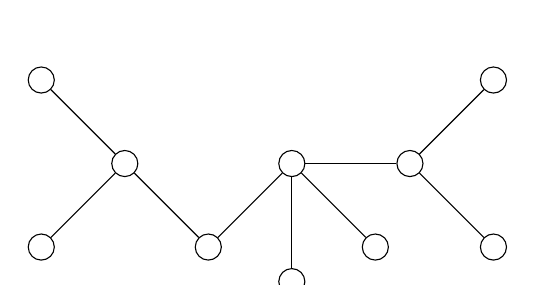
\begin{tikzpicture}[node distance={15mm}, main/.style = {draw, circle}] 
        \node[main] (1) {}; 
        \node[main] (2) [below right of=1] {};
        \node[main] (3) [below left of=2] {}; 
        \node[main] (4) [below right of=2] {};
        \node[main] (5) [above right of=4] {};
        \node[main] (6) [below of=5] {};
        \node[main] (7) [below right of=5] {};
        \node[main] (8) [right of=5] {};
        \node[main] (9) [above right of=8] {};
        \node[main] (10) [below right of=8] {};

        \draw (1) -- (2); \draw (2) -- (3); \draw (2) -- (4);
        \draw (4) -- (5); \draw (5) -- (6); \draw (5) -- (7);
        \draw (5) -- (8); \draw (8) -- (9); \draw (8) -- (10);
    \end{tikzpicture} 
\end{center}
\vspace{-0.25cm}
Given a graph $G = (V, E)$, a {\bf spanning tree} of $G$ is a graph $T = (V, F)$ 
such that $F \subseteq E$ and $T$ is a tree. We illustrate an example of a 
graph $G$ with a subtree $T$ using bold edges below. 
\begin{center}
    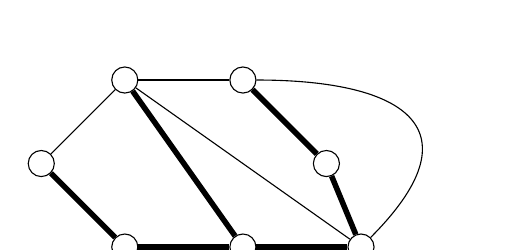
\begin{tikzpicture}[node distance={15mm}, main/.style = {draw, circle}] 
        \node[main] (1) {}; 
        \node[main] (2) [right of=1] {};
        \node[main] (3) [below left of=1] {}; 
        \node[main] (4) [below right of=2] {};
        \node[main] (5) [below right of=3] {};
        \node[main] (6) [right of=5] {};
        \node[main] (7) [right of=6] {};

        \draw (1) -- (2); 
        \draw (1) -- (3); 
        \draw [line width=2pt] (1) -- (6);
        \draw (1) -- (7);
        \draw [line width=2pt] (2) -- (4);
        \draw (2) to [out=0, in=45, looseness=2] (7);
        \draw [line width=2pt] (3) -- (5);
        \draw [line width=2pt] (4) -- (7);
        \draw [line width=2pt] (5) -- (6);
        \draw [line width=2pt] (6) -- (7);
    \end{tikzpicture} 
\end{center}
In an introductory graph theory course, such as MATH 239, 
it is shown that every tree on $n$ vertices has $n-1$ edges. The following 
theorem then gives us a useful characterization of trees. 

\begin{theo}[Fundamental Theorem of Trees]{theo:2.1}
    Let $T = (V, F)$ be a graph. The following are equivalent:
    \begin{enumerate}[(i)]
        \item $T$ is a tree. 
        \item $T$ is connected and $|F| = |V| - 1$. 
        \item $T$ is acyclic and $|F| = |V| - 1$. 
    \end{enumerate}
\end{theo}

In particular, if we know that two of the conditions hold, then the 
third one is guaranteed.

\subsection{Minimum Spanning Trees}\label{subsec:2.2}
Given a connected graph $G = (V, E)$ and edge costs $c_e$ for each 
$e \in E$, our goal is to find a spanning tree $T$ of minimum cost 
\[ c(T) := \sum_{e \in T} c_e. \] 
First, we'll set some notation. For a vertex $v \in V$, we define 
$\delta(v)$ to be the set of edges in $E$ incident to $v$. More generally, 
given a subset of vertices $S \subseteq V$, the {\bf cut induced by $S$} is 
defined to be the set 
\[ \delta(S) := \{uv \in E : u \in S,\, v \notin S\}. \] 
The following theorem will be extremely important for finding a minimum 
spanning tree. 

\begin{theo}[Cut Property]{theo:2.2}
    Suppose that the costs $c_e$ for $e \in E$ are distinct. 
    Let $S \subseteq V$ be such that $S \neq \varnothing$ and $S \neq V$, 
    and let 
    \[ e = \argmin_{f \in \delta(S)} c_f. \] 
    Then every minimum spanning tree contains the edge $e$. 
\end{theo}
\begin{pf}[Theorem~\ref{theo:2.2}]
    We proceed by contradiction. Let $S \subseteq V$ be such that $S 
    \neq \varnothing$ and $S \neq V$, and let $e = \argmin_{f\in S} c_f$. 
    Suppose that there is a minimum spanning tree $T = (V, F)$ such that 
    $e \notin F$. 

    Consider the graph $(V, F \cup \{e\})$. Note that $|F \cup \{e\}| = |V|$ 
    and this graph is connected, so it cannot be a tree by Theorem~\ref{theo:2.1}. 
    In particular, it must contain a cycle $C$. 

    Next, note that $|C \cap \delta(S)|$ must be even because for any 
    edge leaving the cut $\delta(S)$, there must be another edge coming back 
    into the cut. Moreover, since $e \in C \cap \delta(S)$, we have 
    $C \cap \delta(S) \neq \varnothing$. This implies that 
    $|C \cap \delta(S)| \geq 2$, so there is another edge $e' \neq e$ 
    with $e' \in C \cap \delta(S)$.

    Consider now the graph $T' = (V, (F \cup \{e\}) \setminus \{e'\})$. 
    Then $|(F \cup \{e\}) \setminus \{e'\}| = |F| = |V| - 1$ and $T'$ is 
    connected because if a path between two vertices used the edge $e'$, 
    then we could go along the edges in $C \setminus \{e'\}$ instead. 
    So by Theorem~\ref{theo:2.1}, $T'$ is also a spanning tree. 
    Finally, observe that 
    \[ c(T) - c(T') = c_{e'} - c_e > 0 \] 
    because we have $e = \argmin_{f\in S} c_f$ and $e' \neq e$ with 
    $e' \in \delta(S)$, as well as the assumption that the edge 
    costs $c_e$ for $e \in E$ were distinct. But $T'$ has lower cost 
    than $T$, contradicting our assumption that $T$ was a minimum 
    spanning tree. \qed
\end{pf}\vspace{-0.25cm}

The following property relating cycles to minimum spanning trees 
can also be proved similarly to Theorem~\ref{theo:2.2}. 
The main idea is to try to create shortcuts using the edges in the cycle. 

\begin{theo}[Cycle Property]{theo:2.3}
    Let $G = (V, E)$ be connected with distinct edge costs 
    $c_e$ for $e \in E$. Let $C$ be a cycle in $G$ and let 
    \[ e = \argmax_{f\in C} c_f. \] 
    Then no minimum spanning tree contains the edge $e$. 
\end{theo}

\subsection{Prim's Algorithm}\label{subsec:2.3}
Prim's algorithm takes the idea of the cut property (Theorem~\ref{theo:2.2}) 
and uses it to compute a minimum spanning tree starting from an arbitrary 
vertex $s \in V$. At each iteration of the algorithm, we will keep track of a 
set of a partial tree construction $T$ and vertices $A \subseteq V$ that are 
connected to $s$ in $T$. 

\begin{mdframed}[
    linewidth=1pt,
    linecolor=black,
    bottomline=false,topline=false,rightline=false,
    innerrightmargin=0pt,innertopmargin=0pt,innerbottommargin=0pt,
    innerleftmargin=1em,% Distance between vertical rule & proof content
    skipabove=0.75\baselineskip
]
{\bf Input.} A graph $G = (V, E)$ and edge costs $c_e$ for 
all $e \in E$. 

{\bf Output.} A minimum spanning tree of $G$.
\begin{enumerate}[leftmargin=1.75cm, label={Step \arabic*.}]
    \item {\bf Initialization.} Let $s \in V$ be an arbitrary vertex, 
    then set $A \gets \{s\}$ and $T \gets \varnothing$.

    \item While $A \neq V$:
    \begin{enumerate}[label={Step 2.\arabic*.}]
        \item {\bf Pick an edge for the minimum spanning tree.} 
        Set 
        \[ e \gets \argmin_{f \in \delta(A)} c_f, \] 
        where $e = uv$ with $u \in A$ and $v \notin A$.  
        \item {\bf Update values.} Set $A \gets A \cup \{v\}$ and 
        $T \gets T \cup \{e\}$. 
    \end{enumerate}
\end{enumerate}
\end{mdframed}\vspace{-0.15cm}

Let's run Prim's algorithm on a simple example. Consider the following 
graph $G = (V, E)$, and suppose that at Step 1, we pick $v_1$ to be 
the initial vertex. 
\begin{center}
    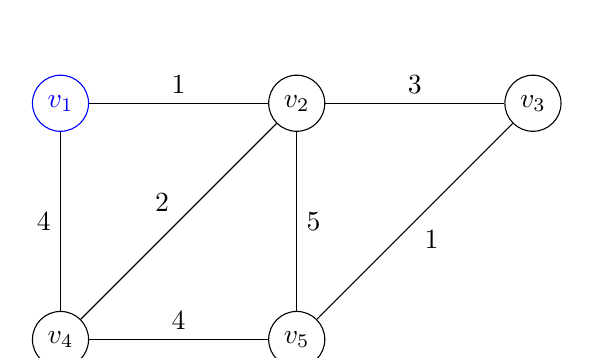
\begin{tikzpicture}[node distance={30mm}, main/.style = {draw, circle}] 
        \node[main, color=blue] (1) {$v_1$}; 
        \node[main] (2) [right of=1] {$v_2$};
        \node[main] (3) [right of=2] {$v_3$}; 
        \node[main] (4) [below of=1] {$v_4$};
        \node[main] (5) [right of=4] {$v_5$};

        \draw (1) -- node[midway, above] {1} (2);
        \draw (2) -- node[midway, above] {3} (3);
        \draw (1) -- node[midway, left] {4} (4);
        \draw (2) -- node[midway, above left] {2} (4);
        \draw (2) -- node[midway, right] {5} (5);
        \draw (3) -- node[midway, below right] {1} (5);
        \draw (5) -- node[midway, above] {4} (4);
    \end{tikzpicture} 
\end{center}
\vspace{-0.25cm}
Then at the first iteration of Step 2.1, we have $\delta(A) = 
\{v_1v_2, v_1v_4\}$, so we pick $e = v_1v_2$ because it has minimum cost.
At Step 2.2, we set $A = \{v_1, v_2\}$ and $T = \{v_1v_2\}$. 

\begin{center}
    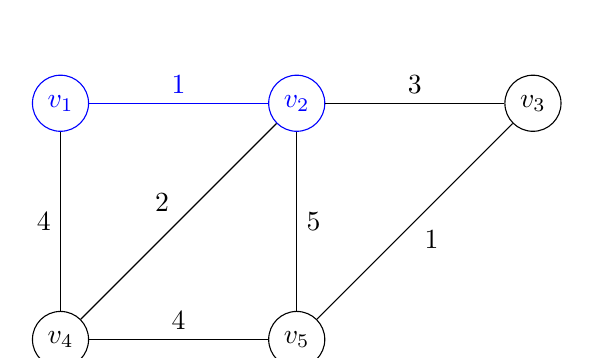
\begin{tikzpicture}[node distance={30mm}, main/.style = {draw, circle}] 
        \node[main, color=blue] (1) {$v_1$}; 
        \node[main, color=blue] (2) [right of=1] {$v_2$};
        \node[main] (3) [right of=2] {$v_3$}; 
        \node[main] (4) [below of=1] {$v_4$};
        \node[main] (5) [right of=4] {$v_5$};

        \draw[color=blue] (1) -- node[midway, above] {1} (2);
        \draw (2) -- node[midway, above] {3} (3);
        \draw (1) -- node[midway, left] {4} (4);
        \draw (2) -- node[midway, above left] {2} (4);
        \draw (2) -- node[midway, right] {5} (5);
        \draw (3) -- node[midway, below right] {1} (5);
        \draw (5) -- node[midway, above] {4} (4);
    \end{tikzpicture} 
\end{center}
\vspace{-0.25cm}
The edge $v_2v_4$ is of minimum cost in the cut induced by $A$, so 
we set $A = \{v_1, v_2, v_4\}$ and $T = \{v_1v_2, v_2v_4\}$ at the next iteration. 
Continuing in this fashion, we obtain the following minimum spanning tree.

\begin{center}
    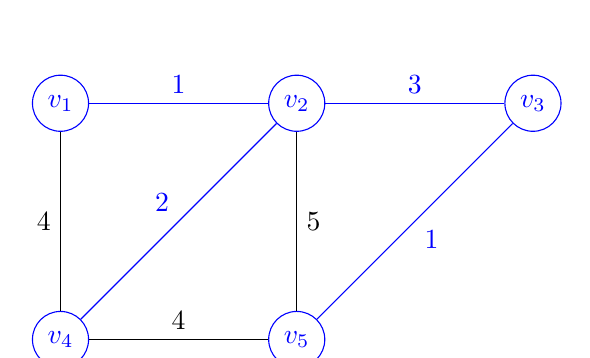
\begin{tikzpicture}[node distance={30mm}, main/.style = {draw, circle}] 
        \node[main, color=blue] (1) {$v_1$}; 
        \node[main, color=blue] (2) [right of=1] {$v_2$};
        \node[main, color=blue] (3) [right of=2] {$v_3$}; 
        \node[main, color=blue] (4) [below of=1] {$v_4$};
        \node[main, color=blue] (5) [right of=4] {$v_5$};

        \draw[color=blue] (1) -- node[midway, above] {1} (2);
        \draw[color=blue] (2) -- node[midway, above] {3} (3);
        \draw (1) -- node[midway, left] {4} (4);
        \draw[color=blue] (2) -- node[midway, above left] {2} (4);
        \draw (2) -- node[midway, right] {5} (5);
        \draw[color=blue] (3) -- node[midway, below right] {1} (5);
        \draw (5) -- node[midway, above] {4} (4);
    \end{tikzpicture} 
\end{center}
\vspace{-0.25cm}
Note that Prim's algorithm may seen similar to Dijkstra's algorithm 
which also yields a spanning tree in the process of computing shortest paths. 
However, these algorithms fundamentally solve different problems, and 
there are examples where the resulting spanning trees do not coincide. 
Moreover, Dijkstra's algorithm takes a directed graph as input, 
whereas Prim's algorithm takes an undirected graph. 

Next, let's prove that Prim's algorithm always gives us a minimum spanning tree. 
For simplicity, we will assume that all edge costs $c_e$ for 
$e \in E$ are distinct. 

\begin{pf}[correctness of Prim's algorithm]
    At every iteration of Step 2, we add one edge to $T$, and we run 
    through $|V| - 1$ iterations. Therefore, $T$ has exactly 
    $|V| - 1$ edges. Moreover, an invariant of Prim's algorithm is that 
    all vertices in $A$ remain connected to $s$, so the final output is 
    also connected. Therefore, we indeed obtain a spanning tree by 
    Theorem~\ref{theo:2.1}. Finally, by the cut property (Theorem~\ref{theo:2.2})
    and our assumption that all the edge costs are distinct, $T$ contains 
    only the edges that are in every minimum spanning tree, so $T$ 
    itself is a minimum spanning tree. \qed 
\end{pf}

As a consequence, we also have the following useful result. 

\begin{cor}{cor:2.4}
    Let $G = (V, E)$ be a connected graph with distinct edge costs $c_e$ for 
    $e \in E$. Then $G$ has a unique minimum spanning tree.
\end{cor}

As usual, let's consider the running time, denoting $|V| = n$ 
and $|E| = m$. For an efficient implementation, 
we keep track of a key $d'(v)$ for each $v \in V \setminus A$. 
Once a vertex $w$ is added to $A$ in Step 2.2, we update the keys via 
$d'(v) \gets \min\{d'(v), c_{wv}\}$ for each $v \in V \setminus A$. 

Note that Step 1 takes $O(1)$ time, and 
there are $n-1$ iterations of Step 2. Implementing Prim's algorithm 
using priority queues, we note that each iteration of Step 2.1 
involves one \textsc{Extract-Min} call, and 
going through all iterations of Step 2.2 takes at most $m$ 
\textsc{Decrease-Key} calls in total. We recall that by using Fibonacci heaps, 
\textsc{Decrease-Key} is $O(1)$ and \textsc{Extract-Min} is $O(\log n)$, 
so we have a total running time of $O(n\log n + m)$. \newpage
\section{Minimum Cost Arborescences}\label{sec:3}

\subsection{Arborescences and a Characterization}\label{subsec:3.1}
Let $G = (V, E)$ be a directed graph and let $r$ be a distinguished 
node, which is commonly called a root. An {\bf arborescence} with respect to 
$r$ (or rooted at $r$) is a directed subgraph $T = (V, F)$ with $F \subseteq E$ 
such that 
\begin{enumerate}[(i)]
    \item undirected $T$ (that is, $T$ obtained from disregarding all directions) is a spanning tree; and 
    \item for every $v \in V$ with $v \neq r$, there is a directed path 
    in $T$ from $r$ to $v$. 
\end{enumerate}
For example, consider the following graph $G = (V, E)$. 
\begin{center}
    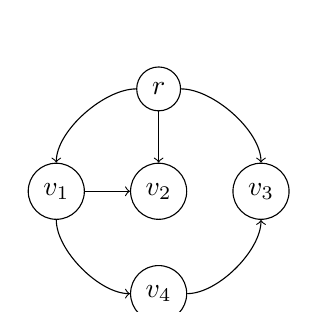
\begin{tikzpicture}[node distance={30mm}, main/.style = {draw, circle}] 
        \node[main] (r) at (0, 1.3) {$r$}; 
        \node[main] (1) at (-1.3, 0) {$v_1$};
        \node[main] (2) at (0, 0) {$v_2$};
        \node[main] (3) at (1.3, 0) {$v_3$};
        \node[main] (4) at (0, -1.3) {$v_4$};

        \draw[->] (r) to [out=180, in=90, looseness=0.75] (1);
        \draw[->] (r) -- (2);
        \draw[->] (r) to [out=0, in=90, looseness=0.75] (3);
        \draw[->] (1) -- (2);
        \draw[->] (1) to [out=270, in=180, looseness=0.75] (4);
        \draw[->] (4) to [out=0, in=270, looseness=0.75] (3);
    \end{tikzpicture} 
\end{center}
\vspace{-0.25cm}
Then the following two subgraphs are arborescences rooted at $r$.
\begin{center}
    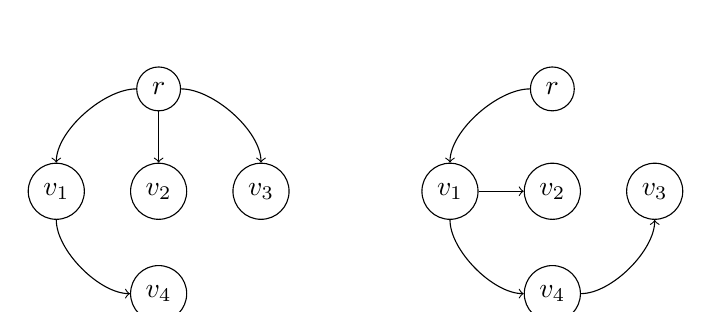
\begin{tikzpicture}[node distance={30mm}, main/.style = {draw, circle}] 
        \node[main] (r) at (0, 1.3) {$r$}; 
        \node[main] (1) at (-1.3, 0) {$v_1$};
        \node[main] (2) at (0, 0) {$v_2$};
        \node[main] (3) at (1.3, 0) {$v_3$};
        \node[main] (4) at (0, -1.3) {$v_4$};

        \node[main] (r') at (5, 1.3) {$r$}; 
        \node[main] (1') at (3.7, 0) {$v_1$};
        \node[main] (2') at (5, 0) {$v_2$};
        \node[main] (3') at (6.3, 0) {$v_3$};
        \node[main] (4') at (5, -1.3) {$v_4$};

        \draw[->] (r) to [out=180, in=90, looseness=0.75] (1);
        \draw[->] (r) -- (2);
        \draw[->] (r) to [out=0, in=90, looseness=0.75] (3);
        % \draw[->] (1) -- (2);
        \draw[->] (1) to [out=270, in=180, looseness=0.75] (4);
        % \draw[->] (4) to [out=0, in=270, looseness=0.75] (3);

        \draw[->] (r') to [out=180, in=90, looseness=0.75] (1');
        % \draw[->] (r') -- (2');
        % \draw[->] (r') to [out=0, in=90, looseness=0.75] (3');
        \draw[->] (1') -- (2');
        \draw[->] (1') to [out=270, in=180, looseness=0.75] (4');
        \draw[->] (4') to [out=0, in=270, looseness=0.75] (3');
    \end{tikzpicture} 
\end{center}
\vspace{-0.25cm}
On the other hand, the following two subgraphs are not arborescences
rooted at $r$: the first one is not a tree, and the second has no directed 
path from $r$ to $v_4$.
\begin{center}
    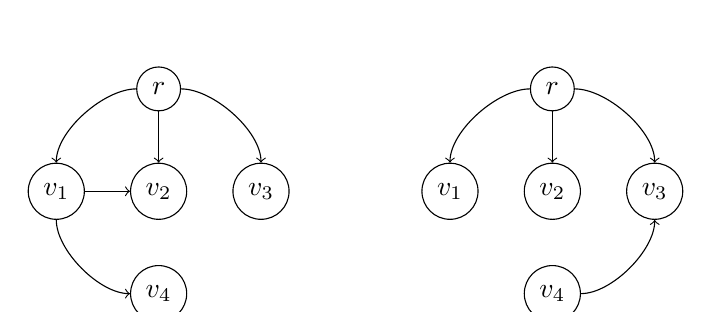
\begin{tikzpicture}[node distance={30mm}, main/.style = {draw, circle}] 
        \node[main] (r) at (0, 1.3) {$r$}; 
        \node[main] (1) at (-1.3, 0) {$v_1$};
        \node[main] (2) at (0, 0) {$v_2$};
        \node[main] (3) at (1.3, 0) {$v_3$};
        \node[main] (4) at (0, -1.3) {$v_4$};

        \node[main] (r') at (5, 1.3) {$r$}; 
        \node[main] (1') at (3.7, 0) {$v_1$};
        \node[main] (2') at (5, 0) {$v_2$};
        \node[main] (3') at (6.3, 0) {$v_3$};
        \node[main] (4') at (5, -1.3) {$v_4$};

        \draw[->] (r) to [out=180, in=90, looseness=0.75] (1);
        \draw[->] (r) -- (2);
        \draw[->] (r) to [out=0, in=90, looseness=0.75] (3);
        \draw[->] (1) -- (2);
        \draw[->] (1) to [out=270, in=180, looseness=0.75] (4);
        % \draw[->] (4) to [out=0, in=270, looseness=0.75] (3);

        \draw[->] (r') to [out=180, in=90, looseness=0.75] (1');
        \draw[->] (r') -- (2');
        \draw[->] (r') to [out=0, in=90, looseness=0.75] (3');
        % \draw[->] (1') -- (2');
        % \draw[->] (1') to [out=270, in=180, looseness=0.75] (4');
        \draw[->] (4') to [out=0, in=270, looseness=0.75] (3');
    \end{tikzpicture} 
\end{center}
\vspace{-0.25cm}
The following theorem gives us a useful characterization of arborescences.

\begin{theo}[Characterization of Arborescences]{theo:3.1}
    Let $G = (V, E)$ be a connected graph and let $T = (V, F)$ be a subgraph. 
    Then $T$ is an arborescence rooted at $r$ if and only if both 
    of the following conditions hold:
    \begin{enumerate}[(1)]
        \item every $v \in V$ with $v \neq r$ has exactly one incoming edge in $T$; and 
        \item $T$ has no directed cycles. 
    \end{enumerate}
\end{theo}
\begin{pf}[Theorem~\ref{theo:3.1}]
    $(\Rightarrow)$ First, we check that condition (1) holds. Consider a vertex 
    $v \in V$ with $v \neq r$. Since undirected $T$ is a spanning tree, 
    there is a unique (simple) path from $r$ to $v$ in undirected $T$. 
    The last edge on this path is incoming for $v$. Hence, all other edges 
    incident to $v$ in undirected $T$ should be outgoing edges for $v$ 
    (because the neighbours of $v$ also have unique simple paths from $v$ 
    to them in undirected $T$). This proves (1). To see that condition (2) 
    holds, note that undirected $T$ is acyclic as it is a spanning tree, 
    so it could not possibly have any directed cycles either. 

    $(\Leftarrow)$ Suppose that $V = (T, F)$ satisfies conditions (1) and (2). 
    First, we show that for all $v \in V$ with $v \neq r$, there exists 
    a directed path from $r$ to $v$ in $T$, which is condition (ii) of the 
    definition of an arborescence. Let $(v_1, v)$ be the unique edge 
    incoming to $v$ by condition (1), let $(v_2, v_1)$ be the unique edge 
    incoming to $v_1$, and so on. By contradiction, suppose that we 
    cannot reach $r$ by backtracking in this way. Then at some point, 
    we must visit the same node at least twice because $G$ is a finite graph. 
    But this creates a directed cycle, contradicting condition (2). Thus, 
    there is a directed path from $r$ to $v$ in $T$. 

    Now, we verify condition (i) that undirected $T$ is a spanning tree. 
    Note that we can get from $r$ to any other vertex $v$, so 
    undirected $T$ is connected. Moreover, $r$ has no incoming edges 
    because if $(v, r)$ is an incoming edge, then the directed path from 
    $r$ to $v$ followed by $(v, r)$ forms a directed cycle, contradicting 
    condition (2). Since every edge is incoming for exactly one of its 
    endpoints, the total number of edges in $T$ is 
    \[ \sum_{u=r} 0 + \sum_{\substack{u\in V \\ u\neq r}} 1 = |V| - 1. \] 
    By the fundamental theorem of trees (Theorem~\ref{theo:2.1}), 
    it follows that undirected $T$ is a spanning tree. \qed 
\end{pf}

\subsection{Minimum Cost Arborescences}\label{subsec:3.2}
Given a directed graph $G = (V, E)$, a distinguished node $r$, and edge 
costs $c_e \geq 0$ for each $e \in E$, our goal is to find an arborescence
rooted at $r$ so that the total edge cost is minimized. 

Let's try to transfer our knowledge from the minimum spanning tree problem. 
Do the analogues of the cycle and cut properties hold for arborescences?
It turns out we can find a counterexample to both in the same graph. 
Consider the following graph $G = (V, E)$ with associated edge costs. 
\begin{center}
    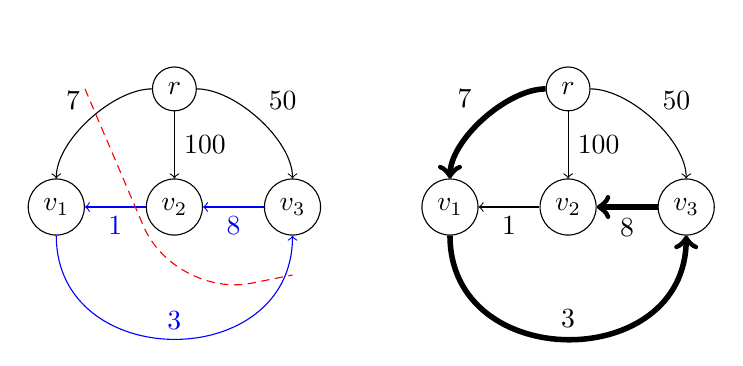
\begin{tikzpicture}[
        node distance={30mm}, 
        main/.style = {draw, circle},
        xs/.style = {xshift=#1 mm},
        ys/.style = {yshift=#1 mm}
    ] 
        \node[main] (r) at (0, 1.5) {$r$}; 
        \node[main] (1) at (-1.5, 0) {$v_1$};
        \node[main] (2) at (0, 0) {$v_2$};
        \node[main] (3) at (1.5, 0) {$v_3$};

        \node[main] (r') at (5, 1.5) {$r$}; 
        \node[main] (1') at (3.5, 0) {$v_1$};
        \node[main] (2') at (5, 0) {$v_2$};
        \node[main] (3') at (6.5, 0) {$v_3$};

        \draw[->] (r) to [out=180, in=90, looseness=0.75] node[midway, above left] {7} (1);
        \draw[->] (r) -- node[midway, right] {100} (2);
        \draw[->] (r) to [out=0, in=90, looseness=0.75] node[midway, above right] {50} (3);
        \draw[->, color=blue] (2) -- node[midway, below] {1} (1);
        \draw[->, color=blue] (3) -- node[midway, below] {8} (2);
        \draw[->, color=blue] (1) to [out=270, in=270, looseness=1.5] node[midway, above] {3} (3);

        \draw[rounded corners=10mm, red, densely dashed] 
            ([xs=-8.5] r.west) -- ([ys=-8] 2.south) -- ([ys=-5] 3.south);

        \draw[->, line width=2pt] (r') to [out=180, in=90, looseness=0.75] node[midway, above left] {7} (1');
        \draw[->] (r') -- node[midway, right] {100} (2');
        \draw[->] (r') to [out=0, in=90, looseness=0.75] node[midway, above right] {50} (3');
        \draw[->] (2') -- node[midway, below] {1} (1');
        \draw[->, line width=2pt] (3') -- node[midway, below] {8} (2');
        \draw[->, line width=2pt] (1') to [out=270, in=270, looseness=1.5] node[midway, above] {3} (3');
    \end{tikzpicture} 
\end{center}
\vspace{-0.25cm}
The minimum cost arborescence is given to the right with cost 
$7 + 3 + 8 = 18$. Consider the cut (in red) and cycle (in blue) above. 
Then the cut property fails to hold because the edge $(v_2, v_1)$ of cost $1$ was 
not picked in a minimum cost arborescence, and the cycle property fails 
to hold because the edge $(v_3, v_2)$ of maximum cost $8$ in the cycle 
was picked in a minimum cost arborescence. 

Can we instead consider the union of minimum cost incoming edges 
(vertex by vertex), excluding the root $r$? For the above example, 
if we start with $v_1$, we'd pick $(v_2, v_1)$ as it is the minimum cost 
edge incoming to $v_1$. Then $(v_1, v_3)$ is the minimum cost edge 
incoming to $v_3$ and $(v_3, v_2)$ is the minimum cost edge incoming to 
$v_2$. This yields the same directed cycle highlighted in blue above!

So this strategy does not immediately work. But if the strategy 
did happen to give us an arborescence, then we are already done! 
All we need to do is tweak it slightly. The idea is to compute 
\[ y_v = \min_{(u,v)\in E} c_{(u, v)} \] 
for all vertices $v \in V$ with $v \neq r$. In particular, any edge using this 
vertex needs to pay this cost anyways. Then for all $(u, v) \in E$, we can 
define new edge costs 
\[ c'_{(u, v)} = c_{(u, v)} - y_v. \] 
We give the edge costs $c'_e$ (in blue) and the values $y_v$ (in purple) for the above example.
Notice that some of the edges turn out to be free.
\begin{center}
    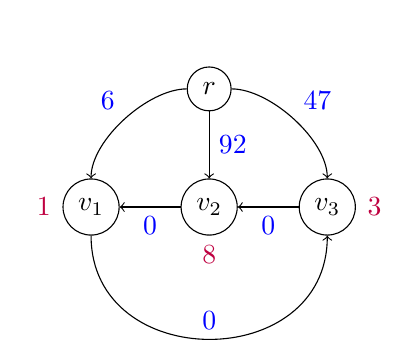
\begin{tikzpicture}[
        node distance={30mm}, 
        main/.style = {draw, circle},
    ] 
        \node[main] (r) at (0, 1.5) {$r$}; 
        \node[main] (1) at (-1.5, 0) {$v_1$};
        \node[color=purple] (1cost) at (-2.1, 0) {$1$};
        \node[main] (2) at (0, 0) {$v_2$};
        \node[color=purple] (2cost) at (0, -0.6) {$8$};
        \node[main] (3) at (1.5, 0) {$v_3$};
        \node[color=purple] (3cost) at (2.1, 0) {$3$};

        \draw[->] (r) to [out=180, in=90, looseness=0.75] node[midway, above left, text=blue] {6} (1);
        \draw[->] (r) -- node[midway, right, text=blue] {92} (2);
        \draw[->] (r) to [out=0, in=90, looseness=0.75] node[midway, above right, text=blue] {47} (3);
        \draw[->] (2) -- node[midway, below, text=blue] {0} (1);
        \draw[->] (3) -- node[midway, below, text=blue] {0} (2);
        \draw[->] (1) to [out=270, in=270, looseness=1.5] node[midway, above, text=blue] {0} (3);
    \end{tikzpicture} 
\end{center}
\vspace{-0.25cm}
Let's prove a useful result regarding these reduced edge costs. Its corollary 
will help us reason about the correctness of a minimum cost arborescence 
algorithm. 

\begin{lemma}{lemma:3.2}
    For every arborescence $T$ rooted at $r$, we have 
    \[ c(T) = c'(T) + \sum_{\substack{v\in V \\ v\neq r}} y_v. \] 
\end{lemma}\vspace{-0.25cm}
\begin{pf}[Lemma~\ref{lemma:3.2}]
    Splitting the sum to correspond to the individual vertices, we have 
    \[ c(T) = \sum_{e\in T} c_e = \sum_{(u, v) \in T} c_{(u,v)} 
    = \sum_{(u, r) \in T} c_{(u,r)} + \sum_{\substack{v\in V\\ v\neq r}} 
    \sum_{(u, v) \in T} c_{(u, v)}. \] 
    There are no edges directed to the root $r$ in an arborescence, so 
    the first sum is $0$. For the double summation, note that in an 
    arborescence, there is exactly one edge directed to each $v \in V$ 
    with $v \neq r$ by Theorem~\ref{theo:3.1}, so we only need to recompensate 
    $y_v$ once. This gives us 
    \begin{align*}
        c(T) &= \sum_{\substack{v\in V\\ v \neq r}} \left( \sum_{(u, v) \in T} (c_{(u, v)} - y_v) + y_v \right) \\
        &= \sum_{\substack{v\in V\\ v \neq r}} \sum_{(u, v) \in T} c'_{(u,v)} + \sum_{\substack{v\in V\\ v \neq r}} y_v 
        = c'(T) + \sum_{\substack{v\in V\\ v \neq r}} y_v,
    \end{align*}
    which is the desired result. \qed
\end{pf}\vspace{-0.25cm}

Since the sum of the vertex costs does not depend on the arborescence 
$T$, we obtain the following corollary. 

\begin{cor}{cor:3.3}
    An arborescence $T$ rooted at $r$ is of minimum cost with respect to 
    edge costs $c_e$ if and only if it is of minimum cost with respect 
    to the reduced edge costs $c'_e$. 
\end{cor}

\subsection{Edmonds' Algorithm}
From the ideas in the previous section, let's build
some intuition for Edmonds' algorithm before we state it. For each $v \neq r$, 
let $f_v = \argmin_{(u, v) \in E} c_{(u, v)}$ be an edge of minimum cost 
entering $v$. Let $F^* = \{f_v : v \neq r\}$ be the set of all of these 
minimum cost edges. Observe that by construction, all edges in $F^*$ have 
reduced edge costs $c'_e = 0$ since they attain the minimum cost 
and we are subtracting that minimum cost afterwards.

If $F^*$ does not contain a cycle, then it is a minimum cost arborescence 
rooted at $r$ by our characterization from Theorem~\ref{theo:3.1} and 
we are done. Otherwise, let $C$ be a cycle in $F^*$. Noting that all 
of the edges in $F^*$ are free with respect to the reduced edge costs, we can 
use as many of these edges as we want. So we can form a new graph 
$G' = (V', E')$ by contracting all the edges in $C$ into a supernode, and 
then recursively solve the problem for $G'$. After solving the problem 
for $G'$, we can extend it to an arborescence for $G$ by adding edges 
from the cycle $C$.

\begin{mdframed}[
    linewidth=1pt,
    linecolor=black,
    bottomline=false,topline=false,rightline=false,
    innerrightmargin=0pt,innertopmargin=0pt,innerbottommargin=0pt,
    innerleftmargin=1em,% Distance between vertical rule & proof content
    skipabove=0.75\baselineskip
]
{\bf Input.} A directed graph $G = (V, E)$, edge costs $c_e \geq 0$ for 
all $e \in E$, and a root node $r$. 

{\bf Output.} A minimum cost arborescence of $G$. 
\begin{enumerate}[leftmargin=1.75cm, label={Step \arabic*.}]
    \item {\bf (Initialization.)} 
    \begin{enumerate}[label={Step 1.\arabic*.}]
        \item {\bf (Find the minimum cost entering each vertex.)} 
        For each $v \in V$ with $v \neq r$, set 
        \begin{align*}
            y_v &\gets \min_{(u, v) \in E} c_{(u, v)}, \\ 
            f_v &\gets \argmin_{(u, v) \in E} c_{(u, v)}. 
        \end{align*}
        \item {\bf (Compute reduced edge costs.)} For each $(u, v) \in E$ 
        where $v \neq r$, set 
        \[ c'_{(u, v)} \gets c_{(u, v)} - y_v. \] 
        \item {\bf (Group edges of minimum cost.)} Set 
        \[ F^* \gets \bigcup_{\substack{v\in V\\ v\neq r}} f_v. \] 
        An equivalent way to see this is that for each $v \neq r$, we are picking 
        one edge $(u, v) \in E$ satisfying $c'_{(u,v)} = 0$.  
    \end{enumerate}

    \item {\bf (Recursive part of the algorithm.)}
    \begin{enumerate}[label={Step 2.\arabic*.}]
        \item {\bf (Base case.)} If $F^*$ is an arborescence rooted at $r$, 
        then stop and output $F^*$.
        \item {\bf (Recursive call.)} Let $C$ be a directed cycle in $F^*$
        (which exists by Theorem~\ref{theo:3.1}). 
        
        Contract $C$ to a supernode to obtain a graph $G' = (V', E')$, keeping 
        the reduced costs $c'_e$. 

        Recursively call Edmonds' algorithm to find a minimum cost arborescence 
        $F'$ for $G'$. Extend $F'$ to an arborescence for $G$ by adding 
        all but one edge in $C$. Then stop and return this arborescence.
    \end{enumerate}
\end{enumerate}
\end{mdframed}\vspace{-0.15cm}
Before we prove correctness, we'll first give a simple example of Edmonds' 
algorithm in action. 

Consider the following graph $G = (V, E)$ with associated edge costs $c_e$. \vspace{-0.15cm}
\begin{center}
    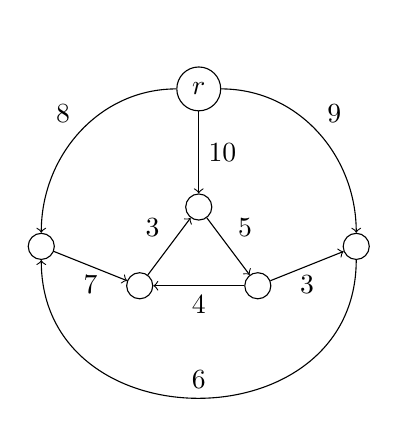
\begin{tikzpicture}[node distance={30mm}, main/.style = {draw, circle}] 
        \node[main] (r) at (0, 1.5) {$r$}; 
        \node[main] (1) at (-2, -0.5) {};
        \node[main] (2) at (0, 0) {};
        \node[main] (3) at (2, -0.5) {};
        \node[main] (4) at (-0.75, -1) {};
        \node[main] (5) at (0.75, -1) {};

        \draw[->] (r) to [out=180, in=90, looseness=1] node[midway, above left] {8} (1);
        \draw[->] (r) -- (2) node[midway, right] {10};
        \draw[->] (r) to [out=0, in=90, looseness=1] node[midway, above right] {9} (3);
        \draw[->] (1) -- node[midway, below] {7} (4);
        \draw[->] (4) -- node[midway, above left] {3} (2);
        \draw[->] (2) -- node[midway, above right] {5} (5);
        \draw[->] (5) -- node[midway, below] {3} (3);
        \draw[->] (5) -- node[midway, below] {4} (4);
        \draw[->] (3) to [out=270, in=270, looseness=1.5] node[midway, above] {6} (1);
    \end{tikzpicture} 
\end{center}
\vspace{-0.85cm}
In Step 1, we compute the minimum cost $y_v$ of entering each vertex $v \neq r$ 
and keep track of a set of edges $F^* = \{f_v : v\neq r\}$ that attain these minimums. 
We then set reduced edge costs $c'_e$. We'll label the edges in $F^*$ in bold, 
the values $y_v$ in purple, and the reduced edge costs $c'_e$ in blue. \vspace{-0.15cm}
\begin{center}
    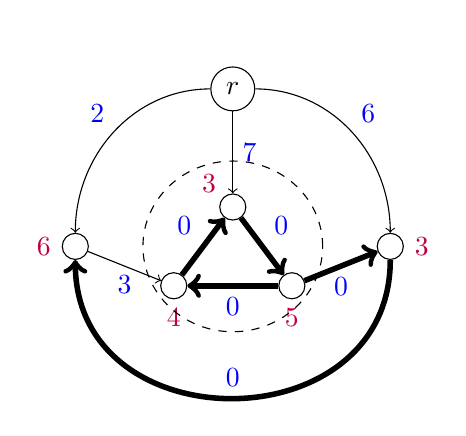
\begin{tikzpicture}[node distance={30mm}, main/.style = {draw, circle}] 
        \node[main] (r) at (0, 1.5) {$r$}; 
        \node[main] (1) at (-2, -0.5) {};
        \node[color=purple] (1cost) at (-2.4, -0.5) {$6$};
        \node[main] (2) at (0, 0) {};
        \node[color=purple] (2cost) at (-0.3, 0.3) {$3$};
        \node[main] (3) at (2, -0.5) {};
        \node[color=purple] (3cost) at (2.4, -0.5) {$3$};
        \node[main] (4) at (-0.75, -1) {};
        \node[color=purple] (4cost) at (-0.75, -1.4) {$4$};
        \node[main] (5) at (0.75, -1) {};
        \node[color=purple] (5cost) at (0.75, -1.4) {$5$};
        \node[draw, dashed, inner sep=0pt, circle, yscale=0.95, fit={(2) (4) (5)}] {};

        \draw[->] (r) to [out=180, in=90, looseness=1] node[midway, above left, text=blue] {2} (1);
        \draw[->] (r) -- (2) node[midway, right, text=blue] {7};
        \draw[->] (r) to [out=0, in=90, looseness=1] node[midway, above right, text=blue] {6} (3);
        \draw[->] (1) -- node[midway, below, text=blue] {3} (4);
        \draw[->, line width=2pt] (4) -- node[midway, above left, text=blue] {0} (2);
        \draw[->, line width=2pt] (2) -- node[midway, above right, text=blue] {0} (5);
        \draw[->, line width=2pt] (5) -- node[midway, below, text=blue] {0} (3);
        \draw[->, line width=2pt] (5) -- node[midway, below, text=blue] {0} (4);
        \draw[->, line width=2pt] (3) to [out=270, in=270, looseness=1.5] node[midway, above, text=blue] {0} (1);
    \end{tikzpicture} 
\end{center}
\vspace{-0.85cm}
We have a directed cycle $C$ in $F^*$ indicated by the 
dotted circle above, so we must proceed to Step 2.2. This step tells us 
to contract $C$ to a supernode to obtain a graph $G' = (V', E')$
with the reduced edge costs $c'_e$. \vspace{-0.15cm}
\begin{center}
    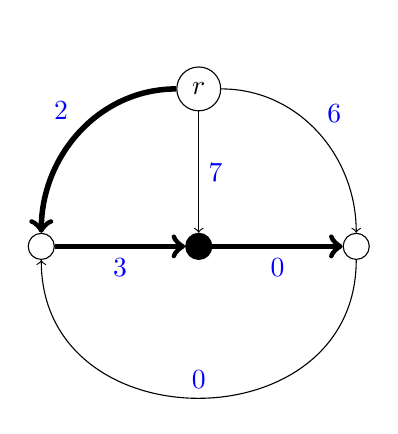
\begin{tikzpicture}[node distance={30mm}, main/.style = {draw, circle}] 
        \node[main] (r) at (0, 1.5) {$r$}; 
        \node[main] (1) at (-2, -0.5) {};
        \node[main] (3) at (2, -0.5) {};
        \node[main, fill=black] (6) at (0, -0.5) {};

        \draw[->, line width=2pt] (r) to [out=180, in=90, looseness=1] node[midway, above left, text=blue] {2} (1);
        \draw[->] (r) -- node[midway, right, text=blue] {7} (6);
        \draw[->] (r) to [out=0, in=90, looseness=1] node[midway, above right, text=blue] {6} (3);
        \draw[->, line width=2pt] (1) -- node[midway, below, text=blue] {3} (6);
        \draw[->, line width=2pt] (6) -- node[midway, below, text=blue] {0} (3);
        \draw[->] (3) to [out=270, in=270, looseness=1.5] node[midway, above, text=blue] {0} (1);
    \end{tikzpicture} 
\end{center}
\vspace{-0.85cm}
Here, we can find by inspection a minimum cost arborescence $F'$ for $G'$ of cost $5$,
highlighted in bold. Now we can extend $F'$ to an arborescence for $G$ 
by adding all but one edge in $C$. \vspace{-0.15cm}
\begin{center}
    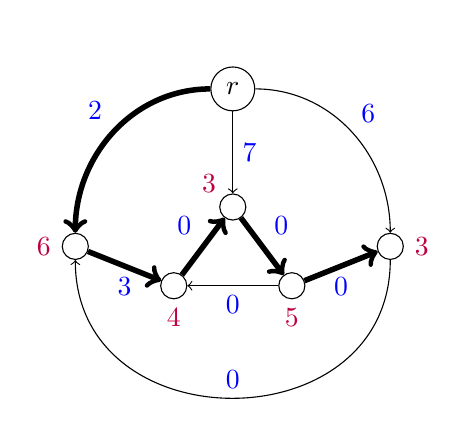
\begin{tikzpicture}[node distance={30mm}, main/.style = {draw, circle}] 
        \node[main] (r) at (0, 1.5) {$r$}; 
        \node[main] (1) at (-2, -0.5) {};
        \node[color=purple] (1cost) at (-2.4, -0.5) {$6$};
        \node[main] (2) at (0, 0) {};
        \node[color=purple] (2cost) at (-0.3, 0.3) {$3$};
        \node[main] (3) at (2, -0.5) {};
        \node[color=purple] (3cost) at (2.4, -0.5) {$3$};
        \node[main] (4) at (-0.75, -1) {};
        \node[color=purple] (4cost) at (-0.75, -1.4) {$4$};
        \node[main] (5) at (0.75, -1) {};
        \node[color=purple] (5cost) at (0.75, -1.4) {$5$};

        \draw[->, line width=2pt] (r) to [out=180, in=90, looseness=1] node[midway, above left, text=blue] {2} (1);
        \draw[->] (r) -- (2) node[midway, right, text=blue] {7};
        \draw[->] (r) to [out=0, in=90, looseness=1] node[midway, above right, text=blue] {6} (3);
        \draw[->, line width=2pt] (1) -- node[midway, below, text=blue] {3} (4);
        \draw[->, line width=2pt] (4) -- node[midway, above left, text=blue] {0} (2);
        \draw[->, line width=2pt] (2) -- node[midway, above right, text=blue] {0} (5);
        \draw[->, line width=2pt] (5) -- node[midway, below, text=blue] {0} (3);
        \draw[->] (5) -- node[midway, below, text=blue] {0} (4);
        \draw[->] (3) to [out=270, in=270, looseness=1.5] node[midway, above, text=blue] {0} (1);
    \end{tikzpicture} 
\end{center}
\vspace{-0.35cm}
Corollary~\ref{cor:3.3} tells us that working with the reduced edge costs 
$c'_e$ still gives us a minimum cost arborescence for the original edge 
costs $c_e$, so Step 1 is valid. 

Moreover, note that the reduced edge costs $c'_e$ are all nonnegative 
and $c'_e = 0$ for all $e \in F^*$, meaning that if $F^*$ happened to be 
an arborescence rooted at $r$ at Step 2.1, then it is an arborescence 
of cost $0$. In particular, every other arborescence also has nonnegative 
cost with respect to $c'_e$, so $F^*$ would be a minimum cost arborescence. 

Arguing the correctness of Step 2.2 is trickier. One concern is that 
contracting the cycle $C$ places extra constraints on the 
arborescence. A minimum cost arborescence in $G'$ must have exactly 
one edge entering the contracted supernode corresponding to $C$. 
However, a minimum cost arborescence for $G$ might have several edges 
entering $C$. To resolve this, we have the following lemma. 

\begin{lemma}{lemma:3.4}
    Let $C$ be a cycle consisting of edges $e$ with $c'_e = 0$, and 
    suppose that $r \notin C$. Then there is a minimum cost arborescence 
    rooted at $r$ that has exactly one edge incoming to $C$.
\end{lemma}\vspace{-0.15cm}
\begin{pf}[Lemma~\ref{lemma:3.4}]
    Let $T$ be a minimum cost arborescence in $G$. By definition, there is a 
    directed $r,v$-path to every vertex $v \neq r$ in $T$, so at least one 
    edge enters $C$. If exactly one edge enters $C$, then we are done by taking $T$. 

    Suppose now that there are at least two edges entering $C$. We will 
    construct another minimum cost arborescence $T'$ that has exactly 
    one edge entering $C$. Let $(u, v)$ be an edge in $T$ entering $C$ 
    that lies on a shortest path from $r$ to $C$. Note that this path from 
    $r$ to $C$ uses only one vertex in $C$. Delete all the edges that 
    enter a vertex in $C$ except for $(u, v)$ from $T$, and add in 
    edges of $C$ except for the one that enters $v$. 

    We claim that $T'$ is a minimum cost arborescence. Note that we are 
    only adding edges with cost $c'_e = 0$, so $c'(T) \geq c'(T')$. 
    By construction, $T'$ has no directed cycles because $T$ had no cycle 
    before and had no cycles within $C$, and now only $(u, v)$ enters $C$. 
    Moreover, there is exactly one edge entering each vertex $v \neq r$ 
    because for every vertex on $C$, we either did nothing or added 
    and removed an edge entering $v$. By Theorem~\ref{theo:3.1}, $T'$ is 
    also a minimum cost arborescence with exactly one edge incoming to $C$. \qed
\end{pf}\vspace{-0.25cm}

Another potential concern: could it be that an arborescence $F'$ rooted at $r$ in the graph 
$G'$ doesn't lead to an arborescence $F$ rooted at $r$ in $G$? It turns 
out that this is impossible; we leave the proof of the following lemma 
as an exercise. The idea is to consider the edges in the cycle $C$, which 
we know have reduced edge costs $c'_e = 0$. 

\begin{lemma}{lemma:3.5}
    Every arborescence $F'$ rooted at $r$ in the graph $G'$ leads to 
    an arborescence $F$ rooted at $r$ in $G$ such that $c'(F') = c'(F)$. 
\end{lemma}\vspace{-0.15cm}
\newpage
\section{Maximum Weight Independent Sets in Matroids}\label{sec:4}

\subsection{Matroids}\label{subsec:4.1}
A {\bf matroid} $M$ is a pair $(S, {\cal I})$ where $S$ is a ground set 
and ${\cal I} \subseteq {\cal P}(S)$ is a family of sets over the 
ground set $S$ satisfying the following properties:
\begin{enumerate}[(1)]
    \item We have $\varnothing \in {\cal I}$.
    \item {\bf Downward closed:} For every $A \in {\cal I}$ and $B \subseteq A$, 
    we have $B \in {\cal I}$. 
    \item {\bf Exchange property:} For every $A, B \in {\cal I}$ with 
    $|A| > |B|$, there exists $e \in A \setminus B$ such that $B \cup \{e\} \in {\cal I}$. 
\end{enumerate}
The sets in the family ${\cal I}$ are called the {\bf independent sets}.

This definition is rather abstract, so we'll go over some examples. 

{\bf Uniform matroids.} Let $S = \{1, \dots, n\}$ and let ${\cal I} = 
\{A \subseteq S : |A| \leq k\}$ for some fixed $k \in \Z^+$. 
\begin{enumerate}[(1)]
    \item We have $\varnothing \in {\cal I}$ since $|\varnothing| = 0 \leq k$. 
    \item If $A \in {\cal I}$ and $B \subseteq A$, then $|B| \leq |A| \leq k$, 
    so $B \in {\cal I}$. 
    \item For every $A, B \in {\cal I}$ with $|A| > |B|$, we have 
    $A \setminus B \neq \varnothing$, so we can pick an element $e \in A 
    \setminus B$. Note that $|B| \leq k-1$, so $|B \cup \{e\}| \leq k$, 
    which implies that $B \cup \{e\} \in {\cal I}$. 
\end{enumerate}

{\bf Partition matroids.} Let $S = \{1, \dots, n\}$ as before, and 
let $S_1, \dots, S_t$ be a partition of $S$. That is, we have 
$\bigcup_{j=1}^t S_j = S$ and $S_i \cap S_j = \varnothing$ whenever 
$i \neq j$. Let ${\cal I} = \{A \subseteq S : |A \cap S_j| \leq r_j 
\text{ for all } j = 1, \dots, t\}$, where $r_j \in \Z^+$ are fixed. 
(Usually, we pick $r_j < |S_j|$, for otherwise this does not put 
any constraints on the independent sets.)
\begin{enumerate}[(1)]
    \item We have $\varnothing \in {\cal I}$ since $|\varnothing \cap S_j| =
    0 \leq r_j$ for all $j = 1, \dots, t$. 
    \item If $A \in {\cal I}$ and $B \subseteq A$, then $|B \cap S_j| 
    \leq |A \cap S_j| \leq r_j$ for all $j = 1, \dots, t$, so $B \in {\cal I}$.
    \item If $A, B \in {\cal I}$ with $|A| > |B|$, then there must exist 
    some $j \in \{1, \dots, t\}$ such that $|A \cap S_j| > |B \cap S_j|$. 
    Then $(A \cap S_j) \setminus (B \cap S_j) \neq \varnothing$, so 
    we can find an element $e \in (A \cap S_j) \setminus (B \cap S_j)$. 
    Observe that 
    \[ |(B \cup \{e\}) \cap S_k| = \begin{cases}
        |B \cap S_k|, & \text{if } k \neq j, \\ 
        |B \cap S_k| + 1, & \text{if } k = j. 
    \end{cases} \] 
    In the first case, we have $|B \cap S_k| \leq r_k$ since $B \in {\cal I}$
    and $e \notin S_k$. For the second case, we have $|B \cap S_j| + 1 
    \leq |A \cap S_j| \leq r_j$ since $A \in {\cal I}$ and 
    $|A \cap S_j| > |B \cap S_j|$. It follows that 
    $B \cup \{e\} \in {\cal I}$. 
\end{enumerate}

The following example is the setting where matroids originated from. 
This is the prototypical example of a matroid given in introductory
talks, and is one we can build our intuition from. 

{\bf Linear matroids.} Let $\mathbb{F}$ be a field. (If you don't remember 
what a field is, it's a set together with two operations satisfying 
some nice axioms; for example, $\mathbb{F} = \mathbb{R}$ is a field under 
the usual addition and multiplication.) 
Let $S$ be a set of vectors in $\mathbb{F}^d$ and let 
${\cal I} = \{A \subseteq S : A \text{ is a linearly independent set over }
\mathbb{F}\}$. Verifying that this is a matroid is an exercise in 
linear algebra, which we won't do here. Such a matroid is said to be 
representable over $\mathbb{F}$.

{\bf Graphic matroids.} Given a graph $G = (V, E)$, let $S = E$, and let 
${\cal I} = \{A \subseteq S : (V, A) \text{ is acyclic}\}$. Then ${\cal I}$ 
consists of all forests (acyclic subgraphs) of $G$.
\begin{enumerate}[(1)]
    \item We see that $(V, \varnothing)$ is acyclic, so $\varnothing \in {\cal I}$. 
    \item If $A \in {\cal I}$ and $B \subseteq A$, then $(V, B)$ has no cycles 
    since $(V, A)$ has no cycles, so $B \in {\cal I}$. 
    \item Let $A, B \in {\cal I}$ with $|A| > |B|$. Then $(V, A)$ has 
    $|V| - |A|$ connected components. Similarly, $(V, B)$ has 
    $|V| - |B|$ connected components, and we have $|V| - |B| > |V| - |A|$. 
    Hence, there is a connected component $C$ of $(V, A)$ that intersects 
    at least two connected components of $(V, B)$, say $C'_1$ and $C'_2$.
    Then $(V, A)$ has a $u, v$-path $P$ where $u \in C'_1$ and 
    $v \in C'_2$. Let $e \in P \cap \delta(C'_1)$, which exists because 
    an edge must cross the boundary of the connected component to 
    get to $C'_2$. Then $B \cup \{e\} \in {\cal I}$.
\end{enumerate}

A maximal independent set $A \in {\cal I}$ is called a {\bf basis}.
It is important to note that maximal is different from maximum. 
Here, we just mean that $A \cup \{e\}$ cannot be independent for any 
$e \in S \setminus A$. 

In the graphic matroid example, the bases correspond to the spanning trees.

Before we move on, we give a few non-examples of matroids. 
\begin{enumerate}[(1)]
    \item Let $S = \{1, 2\}$ and ${\cal I} = \{\{1\}, \{2\}, \{1, 2\}\}$. 
    Then $(S, {\cal I})$ is not a matroid since $\varnothing \notin {\cal I}$. 
    It fails the downward closed property too by considering $\varnothing 
    \subseteq \{1\}$, where $\{1\} \in {\cal I}$.
    \item Let $S = \{1, 2, 3\}$ and ${\cal I} = \{\varnothing, \{1\}, \{2\}, \{3\}, 
    \{1, 2\}\}$. Then $|\{1, 2\}| > |\{3\}|$, but neither $\{1, 3\}$ nor 
    $\{2, 3\}$ are independent sets. Hence, $(S, {\cal I})$ fails the exchange 
    property and is not a matroid.
\end{enumerate}

\begin{lemma}{lemma:4.1}
    All bases for a matroid have the same cardinality.
\end{lemma}\vspace{-0.25cm}
\begin{pf}[Lemma~\ref{lemma:4.1}]
    Let $M = (S, {\cal I})$ be a matroid and let $A, B \in {\cal I}$ be 
    two bases. Suppose by way of contradiction that $|A| > |B|$. 
    Then by the exchange property, we can find $e \in A \setminus B$ 
    such that $B \cup \{e\} \in {\cal I}$, contradicting the maximality of $B$. \qed
\end{pf}\vspace{-0.25cm}

\subsection{Maximum Weight Independent Sets} \label{subsec:4.2}
In the maximum weight independent sets problem, we are given a matroid 
$M = (S, {\cal I})$ and weights $w_e$ for each $e \in S$. The goal 
is to find a maximum weight independent set; that is, a set $A \in {\cal I}$ 
achieving the maximum value of 
\[ w(A) := \sum_{e\in A} w_e. \]
Note that we may assume that $w_e > 0$ for all $e \in S$. Indeed, if 
$A \in {\cal I}$, then by the downward closed property, we have 
$A \setminus \{e \in S : w_e \leq 0\} \in {\cal I}$ as well. But 
\[ w(A \setminus \{e \in S : w_e \leq 0\}) \geq w(A), \] 
so we can simply throw away any elements in $S$ with $w_e \leq 0$ 
and still remain independent.

We now give a greedy algorithm to solve the maximum weight independent 
sets problem under the assumption that $w_e > 0$ for all $e \in S$. 
We notice that it is extremely similar to Kruskal's algorithm.

\begin{mdframed}[
    linewidth=1pt,
    linecolor=black,
    bottomline=false,topline=false,rightline=false,
    innerrightmargin=0pt,innertopmargin=0pt,innerbottommargin=0pt,
    innerleftmargin=1em,% Distance between vertical rule & proof content
    skipabove=0.75\baselineskip
]
{\bf Input.} A matroid $M = (S, {\cal I})$ and weights $w_e > 0$ for all 
$e \in S$.

{\bf Output.} A maximum weight independent set of $M$.
\begin{enumerate}[leftmargin=1.75cm, label={Step \arabic*.}]
    \item Sort the elements in $S$ such that 
    $w_{e_1} \geq w_{e_2} \geq \cdots \geq w_{e_{|S|}}$. 
    Set $A \gets \varnothing$ and $i \gets 1$. 

    \item While $i \neq |S|+1$:
    \begin{enumerate}[label={}]
        \item If $A \cup \{e_i\} \in {\cal I}$, then set $A \gets A \cup \{e_i\}$.
        \item Regardless if we add an element or not, increment $i \gets i+1$.
    \end{enumerate}
\end{enumerate}
\end{mdframed}\vspace{-0.15cm}
It is crucial that we have the assumption $w_e > 0$ for $e \in S$ here, 
because otherwise our greedy algorithm may keep adding negative weight 
elements that keep the set independent, lowering the total weight.

\begin{pf}[correctness of the greedy algorithm]
    Let $A$ denote the output the greedy algorithm. Let $A^*$ be a 
    maximum weight independent set of $M$. It is clear from the construction 
    in Step 2 that $A \in {\cal I}$. Moreover, $A$ is a basis of $M$ 
    because we iterate through every element of $S$ and no element 
    can be further included in $A$ to keep it independent. Similarly, 
    $A^*$ is a basis of $M$. Otherwise, if $A^* \cup \{e\} \in {\cal I}$ 
    for some $e \in S$, then $w(A^* \cup \{e\}) > w(A^*)$ using the 
    assumption that $w_e > 0$, and so $A^*$ was not a maximum weight 
    independent set in the first place. Therefore, we have $|A| = |A^*| = k$ 
    since bases of matroids share the same cardinality by Lemma~\ref{lemma:4.1}.

    Write $A = \{g_1, \dots, g_k\}$ and $A^* = \{g_1^*, \dots, g_k^*\}$ 
    where the elements are sorted such that $w_{g_1} \geq \cdots \geq 
    w_{g_k}$ and $w_{g_1^*} \geq \cdots \geq w_{g_k^*}$. Our aim is to show 
    that $w(A) \geq w(A^*)$. Towards a contradiction, suppose that 
    $w(A) < w(A^*)$ and consider the smallest $j \in \{1, \dots, k\}$ such that 
    \[ w(\{g_1, \dots, g_j\}) < w(\{g_1^*, \dots, g_j^*\}). \] 
    Let $A_{j-1} = \{g_1, \dots, g_{j-1}\}$ and $A_j^* = \{g_1^*, \dots, g_j^*\}$. 
    These are both independent by the downward closed property and we have 
    $|A_j^*| = j > j-1 = |A_{j-1}|$, so it follows by the exchange property 
    that there is some $e \in A_j^* \setminus A_{j-1}$ such that $A_{j-1} 
    \cup \{e\} \in {\cal I}$. Then we obtain 
    \[ w_e \geq w_{g_j}^* > w_{g_j}. \] 
    The first inequality is because $e \in \{g_1^*, \dots, g_j^*\}$ and 
    the edges are sorted by descending weight, and the second inequality 
    is because $w(\{g_1, \dots, g_j\}) < w(\{g_1^*, \dots, g_j^*\})$ 
    while $w(\{g_1, \dots, g_{j-1}\}) \geq w(\{g_1^*, \dots, g_{j-1}^*\})$
    by the way we picked $j$. In particular, let's consider the iteration 
    where $e$ was considered for the greedy algorithm. It must have been 
    before $g_j$ because $w_e > w_{g_j}$. But if $B \cup \{e\} 
    \notin {\cal I}$ for $B \subseteq A_{j-1}$, then $A_{j-1} 
    \cup \{e\} \notin {\cal I}$ as well, which is a contradiction. \qed
\end{pf}\vspace{-0.25cm}

The running time of Step 1 is $O(|S|\log|S|)$ for sorting the elements in $S$. 
In Step 2, there are $|S|$ calls to an independence oracle that tells us 
``yes'' or ``no'' to whether a set is independent, but we do not 
necessarily know the complexity of this oracle. When we discussed Kruskal's 
algorithm, we could efficiently play the role as oracle by using the \textsc{UnionFind} 
data structure, but this is not always the case.

\subsection{Maximum Weight Common Independent Sets} \label{subsec:4.3}
In the maximum weight \emph{common} independent set problem, we are given 
two matroids $M' = (S, {\cal I}')$ and $M'' = (S, {\cal I}'')$ sharing a 
ground set $S$ with weights $w_e$ for $e \in S$. The goal is to find 
a set $A$ such that $A \in {\cal I}'$ and $A \in {\cal I}''$ and 
achieving maximum value 
\[ w(A) = \sum_{e\in A} w_e. \] 
We note that this problem can be solved efficiently with linear programming, 
but we won't state the algorithm here. The extension of this problem 
to even just three matroids becomes NP-hard. For now, we'll give a few 
examples of applications of the two matroid problem. 

{\bf Bipartite matchings.} Let $G = (V, E)$ be a bipartite graph with 
bipartition $(U, W)$. Recall that a bipartite graph is such that 
the vertices are partitioned as $V = U \cup W$, and every edge has 
one endpoint in $U$ and one endpoint in $W$. A {\bf matching} is a set 
of edges $M \subseteq E$ such that for every $v \in V$, we have 
$|M \cap \delta(v)| \leq 1$. In other words, every vertex participates 
in at most one edge. 

Suppose that for a bipartite graph, we want to find a matching $M \subseteq E$
achieving the maximum weight
\[ w(M) = \sum_{e\in M} w_e. \] 
We can formulate this problem as a maximum weight common independent set instance. 
Define matroids $M' = (E, {\cal I}')$ and $M'' = (E, {\cal I}'')$, where 
\begin{align*}
    {\cal I}' &= \{A \subseteq E : |A \cap \delta(u)| \leq 1 \text{ for all } u \in U\}, \\ 
    {\cal I}'' &= \{A \subseteq E : |A \cap \delta(w)| \leq 1 \text{ for all } w \in W\}.
\end{align*}
We see that $\{\delta(u)\}_{u\in U}$ and $\{\delta(w)\}_{w\in W}$ define 
partitions on $E$, and so $M'$ and $M''$ are particular examples of partition 
matroids. Moreover, $M$ is a matching if and only if $M \in {\cal I}'$ and 
$M \in {\cal I}''$. 

{\bf Arborescences.} Let $G = (V, E)$ be a directed graph with edge costs 
$c_e \geq 0$ for all $e \in E$. Let $r \in V$ be a distinguished vertex. 
We can define matroids $M' = (E, {\cal I}')$ 
and $M'' = (E, {\cal I}'')$ where 
\begin{align*}
    {\cal I}' &= \{A \subseteq E : (V, A) \text{ is acyclic when ignoring directions}\}, \\ 
    {\cal I}'' &= \{A \subseteq E : |\delta^{\text{in}}(v) \cap A| \leq 1 - \delta_{vr} \text{ for all } v \in V\}.
\end{align*}
Here, $\delta^{\text{in}}(v)$ denotes the set of edges incoming to $v$, 
and $\delta_{vr}$ is the Kronecker delta so that 
\[ 1 - \delta_{vr} = \begin{cases}
    1, & \text{if } v \neq r, \\ 
    0, & \text{if } v = r.
\end{cases} \] 
We see that $M' = (E, {\cal I}')$ is a graphic matroid and $M'' = 
(E, {\cal I}'')$ is a partition matroid, with $T$ being an arborescence 
rooted at $r$ if and only if $T$ is a basis for both $M'$ and $M''$. \newpage
\section{Minimum Cost Steiner Trees} \label{sec:5}

\subsection{Minimum Steiner Tree Problem}
Given an (undirected) graph $G = (V, E)$, edge costs $c_e \geq 0$ for all 
$e \in E$, and {\bf terminals} $T \subseteq V$, the goal is to find a 
minimum cost tree that connects all the terminals in $T$. For example, 
the vertices in blue below denote the terminals $T \subseteq V$, 
and the bold edges form a Steiner tree connecting the terminals in $T$. 
\begin{center}
    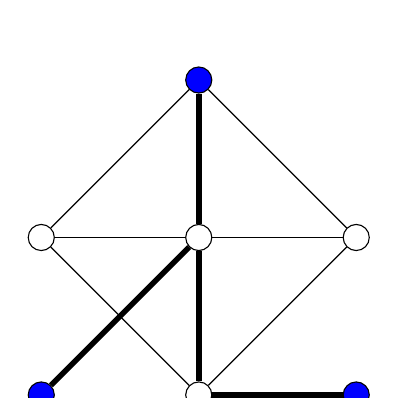
\begin{tikzpicture}[node distance={30mm}, main/.style = {draw, circle}] 
        \node[main, fill=blue] (1) at (2, 4) {}; 
        \node[main] (2) at (0, 2) {};
        \node[main] (3) at (2, 2) {};
        \node[main] (4) at (4, 2) {};
        \node[main, fill=blue] (5) at (0, 0) {};
        \node[main] (6) at (2, 0) {};
        \node[main, fill=blue] (7) at (4, 0) {};

        \draw (1) -- (2);
        \draw[line width=2pt] (1) -- (3);
        \draw (1) -- (4);
        \draw (2) -- (3);
        \draw (2) -- (6);
        \draw (3) -- (4);
        \draw[line width=2pt] (3) -- (5);
        \draw[line width=2pt] (3) -- (6);
        \draw (4) -- (6);
        \draw[line width=2pt] (6) -- (7);
    \end{tikzpicture} 
\end{center}
\vspace{-0.25cm}
Note that we have already seen some particular instances of this problem before.
\begin{itemize}
    \item If $T$ is empty or consists of a single vertex, then this problem is 
    trivial; just don't take any edges.
    \item If $|T| = 2$, then this is the shortest path problem.
    \item If $T = V$, then this is the minimum spanning tree problem.
\end{itemize}
However, it turns out that this problem is $\NP$-hard in general!

\subsection{Minimum Metric Steiner Tree Problem} \label{subsec:5.2}
This problem is a minimum Steiner tree problem where we impose the additional 
conditions that
\begin{enumerate}[(a)]
    \item $G = (V, E)$ is complete; and 
    \item $c_{uw} \leq c_{uv} + c_{vw}$ for all distinct $u, v, w \in V$.
\end{enumerate}
Since the edge costs satisfy the triangle inequality, we are living 
in a metric space in some sense, which explains the name of the problem.

It turns out that these problems are equivalent, even though the metric 
version looks like a much more specific case than the original version! 
In our reluctance to call this the \textsc{MST} problem due to minimum 
spanning trees, let's call them \textsc{MSteinerT} and \textsc{MMSteinerT}
respectively. 

If we have an oracle for \textsc{MSteinerT}, then given an instance of 
\textsc{MMSteinerT}, we can simply feed it to the oracle for \textsc{MSteinerT}
as it solves the more general problem. The hard part of the equivalence 
is proving the other direction where if we have an oracle for 
\textsc{MMSteinerT}, then we can also solve \textsc{MSteinerT} efficiently.

Suppose we are given an instance of \textsc{MSteinerT} $(G, c, T)$, 
where $G = (V, E)$. Consider $(G', c', T')$, where
\begin{itemize}
    \item $T' = T$;
    \item $G' = (V, E')$ is the complete graph on the vertices of $G$; and 
    \item $c'_{uv}$ is the length of a shortest $u,v$-path in $G$ with 
    respect to edge costs $c_e$.
\end{itemize}
The following lemma tells us that $(G', c', T')$ is in fact an instance of 
\textsc{MMSteinerT}.

\begin{lemma}{lemma:5.1}
    \begin{enumerate}[(a)]
        \item For every Steiner tree $F$ for the instance 
        $(G, c, T)$, $F' = F$ is also a Steiner tree for the 
        instance $(G', c', T')$ of cost 
        $c'(F') \leq c(F)$. 
        \item For any Steiner tree $F'$ for the instance 
        $(G', c', T')$, there is a Steiner tree $F$ for the 
        instance $(G, c, T)$ such that $c(F) \leq c'(F')$. 
        \item The new edge costs $c'$ satisfy the triangle inequality. In particular, 
        $(G', c', T')$ is an instance of \textsc{MMSteinerT}.
    \end{enumerate}
\end{lemma}\vspace{-0.25cm}
\begin{pf}[Lemma~\ref{lemma:5.1}]
    \begin{enumerate}[(a)]
        \item Since $E' \supseteq E$, we have that $F \subseteq E'$. Moreover, 
        $F$ is still a tree and connects all vertices in $T = T'$. Note that 
        for every edge $e \in E$, we have $c'_e \leq c_e$ because 
        taking the edge $e = uv$ is among one possibility for a $u,v$-path
        and $c'_e$ corresponds to the length of the shortest one. This 
        gives us $c'(F) \leq c(F)$. 
        \item For each $uv \in F'$, consider a shortest $u, v$-path 
        $P_{uv}$ in the original instance $(G, c, T)$. Let 
        \[ K = \bigcup_{uv \in F'} P_{uv} \] 
        be the union of all the edges in these shortest paths. (Note that 
        $K$ is not necessarily a tree.) Since $c(P_{uv}) \leq c'_{uv}$ 
        by construction, we have 
        \[ c(K) \leq c'(F') = \sum_{uv \in F'} c'_{uv}. \]
        Also, $K$ consists only of edges in the original graph $G$ and 
        connects all terminals in $T$. Consider the subgraph  
        with $K$ as the edges and look at the connected component containing 
        the terminals in $T$. Construct a spanning tree $F$ on this connected 
        component. Then $c(F) \leq c(K) \leq c'(F')$ and $F$ connects 
        the terminals in $T$, so it is a Steiner tree for $(G, c, T)$. 
        \item Let $u, v, w \in V$ be distinct. Consider a shortest $u,v$-path 
        $P_1$, a shortest $v,w$-path $P_2$, and a shortest $u,w$-path $P_3$ 
        in $G$ with respect to the original costs $c$. By definition, we have 
        $c'_{uv} = c(P_1)$, $c'_{vw} = c(P_2)$, and $c'_{uw} = c(P_3)$. 
        Note that $P_1$ together with $P_2$ yields a $u,w$-path. Since $P_3$ 
        is a shortest $u,w$-path, it cannot be more expensive than 
        the aforementioned $u,w$-path, so we obtain 
        \[ c'_{uv} + c'_{vw} = c(P_1) + c(P_2) \geq c(P_3) = c'_{uw}, \] 
        so the triangle inequality holds. \qed
    \end{enumerate} 
\end{pf}\vspace{-0.25cm}
Therefore, given an \textsc{MSteinerT} instance, we can efficiently construct 
an \textsc{MMSteinerT} instance. Moreover, if $\textsf{OPT}$ is an optimal solution for 
$(G, c, T)$ and $\textsf{OPT}'$ is an optimal solution for $(G', c', T')$, 
then $c(\textsf{OPT}) \geq c'(\textsf{OPT}')$ by part (a) of Lemma~\ref{lemma:5.1},
and $c'(\textsf{OPT}') \geq c(\textsf{OPT})$ by part (b). This gives us 
$c(\textsf{OPT}) = c'(\textsf{OPT}')$,
so given an oracle to solve \textsc{MMSteinerT}, we can also solve 
\textsc{MSteinerT} instances efficiently by creating a new instance 
of \textsc{MMSteinerT} and feeding it as input to the oracle.

\subsection{An Approximation Algorithm for the Metric Problem} \label{subsec:5.3}
Let's now try to solve \textsc{MMSteinerT} for a given instance $(G', c', T')$;
that is, $G'$ is a complete graph and the costs $c'$ satisfy the triangle 
inequality. Unfortunately, since \textsc{MSteinerT} is $\NP$-hard, so is 
\textsc{MMSteinerT}, because these problems are equivalent! As such, we don't 
know how to solve it efficiently. If there is an efficient algorithm to solve it, this 
shows that $\Poly = \NP$, resolving the major million dollar problem!

Although we can't find the optimal solution efficiently, we can get an 
approximate solution that isn't too far from optimal in polynomial time. 
Consider the {\bf induced subgraph} of $G'$ on the vertices $T'$, given by 
\[ G'[T'] = (T', \{uv : u, v \in T' \text{ with } u\neq v\}), \] 
which is the complete graph on the vertices in $T'$. The idea is to find a 
minimum spanning tree $F''$ in $G'[T']$ with respect to the costs $c'$. 
We have already seen that this can be done in polynomial time by using 
Prim's algorithm or Kruskal's algorithm. Note that $F''$ is a Steiner 
tree of $(G', c', T')$ of cost $c'(F'')$. 

We cannot hope that $F''$ is an optimal solution in general. For example, 
consider the complete graph $G' = (V', E')$, and let $u \in V'$. Set 
$T' = V' \setminus \{u\}$, and define edge costs by 
\[ c'_{vw} = \begin{cases}
    1, & \text{if } v=u \text{ or } w=u, \\ 
    2, & \text{otherwise.}
\end{cases} \] 
It can be checked that these satisfy the triangle inequality. We illustrate 
this graph below when $|T'| = 3$. 
\begin{center}
    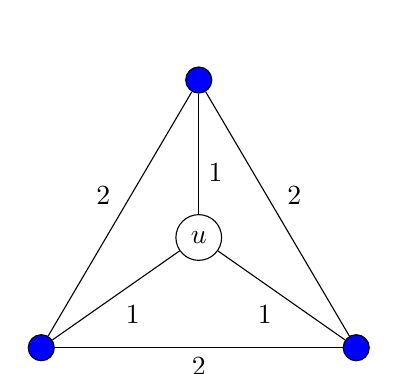
\begin{tikzpicture}[node distance={30mm}, main/.style = {draw, circle}] 
        \node[main] (u) at (0, 0) {$u$}; 
        \node[main, fill=blue] (1) at (0, 2) {};
        \node[main, fill=blue] (2) at (-2, -1.4) {};
        \node[main, fill=blue] (3) at (2, -1.4) {};

        \draw (u) -- (1) node[midway, below right] {1};
        \draw (u) -- (2) node[midway, below right] {1};
        \draw (u) -- (3) node[midway, below left] {1};
        \draw (1) -- (2) node[midway, above left] {2};
        \draw (1) -- (3) node[midway, above right] {2};
        \draw (2) -- (3) node[midway, below] {2};
    \end{tikzpicture} 
\end{center}\vspace{-0.25cm}
For this graph, we see that the optimal solution has value $c(\textsf{OPT}') = 
|T'|$ by taking all the edges with $u$ as an endpoint with cost $1$. 
On the other hand, the induced subgraph $G'[T']$ does not contain $u$, 
so a minimum spanning tree takes only the edges of cost $2$, and there are 
$|T'| - 1$ of them. Therefore, we have 
\[ c'(F'') = 2(|T'| - 1) > |T'| = c(\textsf{OPT}') \] 
when $|T'| \geq 3$, and as $|T'| \to \infty$, we see that 
\[ \frac{c'(F'')}{c'(\textsf{OPT}')} = \frac{2(|T'| - 1)}{|T'|} \to 2. \] 
Fortunately, when using this strategy, this error is the worst it could get.

\begin{lemma}{lemma:5.2}
    Let $F''$ be a minimum spanning tree for $G'[T']$, and let $\textsf{OPT}'$ be 
    an optimal solution for $(G', c', T')$. Then $c'(F'') \leq 2c'(\textsf{OPT}')$.
\end{lemma}\vspace{-0.25cm}
\begin{pf}[Lemma~\ref{lemma:5.2}]
    Let $P$ be an Euler tour on the optimal solution $\textsf{OPT}'$, which is 
    a Steiner tree. That is, $P$ is a path where the starting vertex is 
    the same as the finish vertex, and it visits all the terminals in $T'$.
    Note that $P$ uses every edge in $\textsf{OPT}'$ exactly twice, so 
    $c'(P) = 2c'(\textsf{OPT}')$. Let 
    \[ F^* := \{uv : u, v \in T' \text{ where } u \text{ and } v \text{ 
        are consecutive terminals on the tour $P$}\}. \] 
    Then $F^*$ is a set of edges in $G'[T']$. For every edge $uv \in F^*$, 
    we have by the triangle inequality that 
    \[ c'_{uv} \leq c'(P_{uv}), \] 
    where $P_{uv}$ is the part of the Euler tour 
    $P$ between $u$ and $v$. This gives 
    \[ \sum_{e\in F^*} c'_e \leq c'(P) = 2c'(\textsf{OPT}'). \] 
    Note that $F^*$ connects all the vertices in $G'[T']$ since $P$ connects 
    all the vertices in $T'$. Thus, $G'[T']$ has a spanning tree $\overline{F}$ 
    such that $\overline{F} \subseteq F^*$, so $c'(\overline{F}) \leq 
    2c'(\textsf{OPT}')$. But $F''$ is a minimum spanning tree of $G'[T']$, 
    so we deduce that $c'(F'') \leq c'(\overline{F}) \leq 2c'(\textsf{OPT}')$. \qed
\end{pf}\vspace{-0.25cm}
Let $\alpha \geq 1$. An {\bf $\alpha$-approximation algorithm} for a minimization problem is an 
algorithm that outputs a feasible solution with value at most 
$\alpha \cdot z(\textsf{OPT})$, where $z$ denotes the objective 
function and $\textsf{OPT}$ is an optimal solution 
for the minimization problem.

Similarly, for $\alpha \leq 1$, an $\alpha$-approximation algorithm for a 
maximization problem outputs a feasible solution with 
value at least $\alpha \cdot z(\textsf{OPT})$, where $z$ is the objective 
function and $\textsf{OPT}$ is an optimal solution 
for the maximization problem.

From Lemma~\ref{lemma:5.2}, we see that the following is an efficient 
$2$-approximation algorithm for $\textsc{MMSteinerT}$.

\begin{mdframed}[
    linewidth=1pt,
    linecolor=black,
    bottomline=false,topline=false,rightline=false,
    innerrightmargin=0pt,innertopmargin=0pt,innerbottommargin=0pt,
    innerleftmargin=1em,% Distance between vertical rule & proof content
    skipabove=0.75\baselineskip
]
{\bf Input.} A complete graph $G = (V, E)$, costs $c_e \geq 0$ for each $e \in E$ 
satisfying the triangle inequality, and terminals $T \subseteq V$. 

{\bf Output.} A minimum cost Steiner tree connecting the terminals in $T$.
\begin{enumerate}[leftmargin=1.75cm, label={Step \arabic*.}]
    \item Construct the induced subgraph $G[T]$.
    \item Compute a minimum spanning tree $F''$ in $G[T]$ and output $F''$.
\end{enumerate}
\end{mdframed}\vspace{-0.35cm}
We will say more on approximation algorithms later. Before that, we will 
discuss some complexity theory in the next section.\newpage
\section{Complexity Theory} \label{sec:6}

\subsection{The Complexity Class $\Poly$} \label{subsec:6.1}
The complexity class $\Poly$ consists of all problems that can be solved
efficiently (in polynomial time). 
\begin{itemize}
    \item The problem $\textsc{MST}$ of finding a minimum spanning tree is in $\Poly$ 
    using Prim's or Kruskal's algorithm. 
    \item The problem $\textsc{ShortestPaths}$ is in $\Poly$ using Dijkstra's algorithm.
    \item The problem $\textsc{MCA}$ of finding a minimum cost arborescence is in 
    $\Poly$ by using Edmonds' algorithm. 
    \item However, we are unsure whether or not $\textsc{MSteinerT}$ and $\textsc{MMSteinerT}$
    are in $\Poly$. We'll discuss this further when we introduce the class $\NP$.
\end{itemize}

Let $X$ be a minimization problem. The {\bf decision problem} corresponding 
to $X$ takes as input an instance of $X$ and a number $k$, and answers 
if there is a feasible solution for the given instance of value at most $k$. 

For example, the decision version of the $\textsc{MSteinerT}$ problem, 
which we'll call $\textsc{DecisionMSteinerT}$, takes as input a graph 
$G = (V, E)$, costs $c_e \geq 0$ for $e \in E$, terminals $T \subseteq V$, 
and a number $k$. To solve the problem, we should output ``yes'' if there 
exists a Steiner tree of cost at most $k$, and output ``no'' otherwise. 

We'll be working with linear programs a lot later in this course. Therefore, 
we should note that solving a linear program is in $\Poly$. 
\begin{itemize}
    \item It is still not known whether the simplex algorithm can be implemented 
    to give a polynomial running time in the worst case. The hard part is the choice of 
    the pivoting rule; it is known that Bland's rule, which ensures that 
    the simplex algorithm never cycles, is quite inefficient.
    \item There are other algorithms that can solve linear programs in 
    polynomial time. The first one to be discovered was the ellipsoid method, 
    but it is also inefficient in practice. 
\end{itemize} 

\subsection{Polynomial Time Reductions} \label{subsec:6.2}
We have seen a glimpse of reductions when we discussed 
$\textsc{MSteinerT}$ and $\textsc{MMSteinerT}$ in Section~\ref{subsec:5.2}. 
Given two problems $X$ and $Y$, we say that $X$ {\bf reduces} in polynomial 
time to $Y$, denoted by $X \leq_P Y$, if one can solve $X$ by using a 
polynomial number of basic operations and a polynomial number of calls 
to an oracle that solves $Y$. Intuitively, this means that $X$ is ``not 
harder'' than $Y$, because if we know how to solve $Y$, then we have 
a way to solve $X$. We look at some examples of reductions.
\begin{itemize}
    \item We can show that $\textsc{MST} \leq_P \textsc{MSteinerT}$. 
    Suppose we are given an instance of $\textsc{MST}$, namely a graph 
    $G = (V, E)$ and edge costs $c_e$ for each $e \in E$. Then we can 
    construct an instance of $\textsc{MSteinerT}$ by simply setting 
    $T = V$. We can pass $(G, c, T)$ to an oracle that solves $\textsc{MSteinerT}$
    and output that result. 
    Overall, this process involved a polynomial number of operations 
    (assigning $T = V$), and then a polynomial number of calls to 
    the oracle (only one call was needed here).

    \item Next, let's show that $\textsc{MST} \leq_P \textsc{MCA}$. As before, 
    suppose we are given an instance of $\textsc{MST}$, so a graph $G = (V, E)$ 
    and edge costs $c_e$ for each $e \in E$. We now construct 
    an instance of $\textsc{MCA}$ as follows. Let $r$ be an 
    arbitrary node in $V$. Let $G' = (V', E')$ where 
    $V' = V$ and 
    \[ E' = \{(u, v) : uv \in E\} \cup \{(v, u) : uv \in E\}. \] 
    Set edge costs $c'_{(u,v)} = c'_{(v,u)} = c_{uv}$ for all $uv \in E$.
    Feed this instance $(G', c', r)$ of $\textsc{MCA}$ to the oracle that 
    solves it and output the obtained arborescence, ignoring directions.
\end{itemize}
However, these reductions were a bit silly. We already know that we can solve 
$\textsc{MST}$ in polynomial time; we didn't even need the oracles for the 
other problems! In particular, any problem in $\Poly$ reduces to 
any other problem simply by using the polynomial time algorithm that solves it.

Suppose that $X$ and $Y$ are problems such that $X \leq_P Y$. We make two 
easy observations: 
\begin{itemize}
    \item If $Y \in \Poly$, then $X \in \Poly$ because adding a polynomial 
    to a product of polynomials is still a polynomial. 
    \item If $X \notin \Poly$, then $Y \notin \Poly$. This is just the 
    contrapositive of the previous point, but this statement 
    is slightly more interesting. 
\end{itemize}
Moreover, if $X \leq_P Y$ and $Y \leq_P Z$, then $X \leq_P Z$ since the composition 
of polynomials is a polynomial.

\subsection{The Complexity Class $\NP$} \label{subsec:6.3}
Let $X$ be a decision problem. An {\bf efficient certifier} $B$ for the 
problem $X$ is an algorithm with polynomial running time which takes 
two inputs $s$ and $t$, where $s$ is an instance of $X$ and $t$ is a 
{\bf certificate}. 
\begin{itemize}
    \item If $s$ is a ``yes'' instance of $X$, then there exists a certificate 
    $t$ whose size is polynomial in the size of $s$ such that $B(s, t)$ 
    returns ``yes''.
    \item If $s$ is a ``no'' instance of $X$, then $B(s, t)$ returns ``no'' 
    for all certificates $t$. 
\end{itemize}
Recall that the $\textsc{DecisionMSteinerT}$ problem takes as input a 
graph $G = (V, E)$, costs $c_e \geq 0$ for $e \in E$, terminals $T \subseteq V$, 
and a number $k$. This is a ``yes'' instance if there exists a Steiner tree 
of cost at most $k$, and a ``no'' instance otherwise. 

For this problem, 
a certificate $t$ is an edge set $F$, and the efficient certifier 
outputs ``yes'' if $F$ is a Steiner tree with $c(F) \leq k$, and outputs ``no'' 
otherwise. For checking that $F$ is a Steiner tree, it needs to verify that 
the edges form a  tree and the terminals are all connected, both of which can be 
done in polynomial time.

The complexity class $\NP$ is the class of all decision problems that admit 
an efficient certifier. In other words, $\NP$ consists of problems where 
``yes'' instances can be verified efficiently with a ``short'' certificate.

Clearly, if a decision problem is in $\Poly$, then it is in $\NP$. 
The verifier can use the polynomial time algorithm that solves the 
decision problem and completely ignore the certificate.
Conversely, it is not known whether every decision problem in $\NP$ 
also lies in $\Poly$. This is the famous $\Poly = \NP$ problem. 

\subsection{$\NP$-hardness and $\NP$-completeness} \label{subsec:6.4}
A problem $X$ is said to be {\bf $\NP$-hard} if for every problem $Y \in \NP$, 
we have $Y \leq_P X$. Furthermore, we say that $X$ is {\bf $\NP$-complete} if $X \in \NP$ 
and $X$ is $\NP$-hard. We can think of $\NP$-complete problems as the 
``hardest problems in $\NP$''.

In the $\textsc{3-SAT}$ problem, we are given boolean variables $x_1, \dots, x_n$ and clauses 
$C_1, \dots, C_k$ that are disjunctions of the form $t_1 \vee t_2 \vee t_3$ 
where $t_1, t_2, t_3 \in \{x_1, \dots, x_n\} \cup \{\overline{x_1}, \dots, \overline{x_n}\}$. 
The goal is to determine if there is a truth assignment to the boolean variables 
$x_1, \dots, x_n$ such that $C_1 \wedge C_2 \wedge \cdots \wedge C_k$ is satisfied. 

For example, given the variables $x_1, x_2, x_3, x_4$ and the clauses 
\[ (x_1 \vee \overline{x_2} \vee x_3) \wedge (\overline{x_1} \vee x_2 \vee x_4) 
\wedge (\overline{x_1} \vee \overline{x_3} \vee \overline{x_4}), \] 
we see that the assignment $x_1 = x_2 = \textsf{False}$ and 
$x_3 = x_4 = \textsf{True}$ does the trick.

The $\textsc{3-SAT}$ problem is one of the most famous in computer science 
because it is one of the first problems shown to be $\NP$-complete, 
due to Cook and Levin in 1973.

\begin{theo}[Cook-Levin]{theo:6.1}
    $\textsc{3-SAT}$ is $\NP$-complete.
\end{theo}

There has been a lot of growth in computational complexity theory in 
the past few decades, so we now have a large variety of $\NP$-complete 
problems to work with. To prove that a given problem $X$ is $\NP$-complete, 
it suffices to do the following: 
\begin{enumerate}[(i)]
    \item Show that $X \in \NP$. This part is typically easy to prove. 
    \item Find another $\NP$-complete problem $Y$ and show that $Y \leq_P X$. 
    This will imply that $X$ is $\NP$-hard because we have $Z \leq_P Y$ for all 
    $Z \in \NP$ and hence $Z \leq_P X$ by transitivity.
\end{enumerate}
We now take a look at the decision vertex cover problem, which we denote by
\textsc{DecVC}. Here, we are given a graph $G = (V, E)$ and a number 
$\ell$. The goal is to determine whether if there is a vertex set $U \subseteq V$ 
such that $|U| \leq \ell$ and every edge $e \in E$ has at least one 
endpoint in $U$.

For example, the following graph has the vertex cover in blue with $\ell = 3$.
\begin{center}
    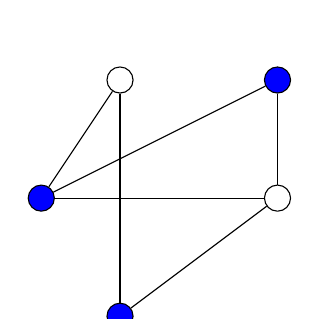
\begin{tikzpicture}[node distance={30mm}, main/.style = {draw, circle}] 
        \node[main] (1) at (4, 2) {}; 
        \node[main, fill=blue] (2) at (6, 2) {};
        \node[main, fill=blue] (3) at (3, 0.5) {};
        \node[main] (4) at (6, 0.5) {};
        \node[main, fill=blue] (5) at (4, -1) {};

        \draw (1) -- (3); \draw (1) -- (5); \draw (2) -- (3);
        \draw (2) -- (4); \draw (3) -- (4); \draw (4) -- (5);
    \end{tikzpicture} 
\end{center}\vspace{-0.25cm}
On the other hand, the complete graph $K_5$ has no vertex cover with size 
at most $\ell = 3$. 

\begin{prop}{prop:6.2}
    \textsc{DecVC} is $\NP$-complete.
\end{prop}\vspace{-0.25cm}
\begin{pf}[Proposition~\ref{prop:6.2}]
    We use the recipe that we supplied above. First, we show 
    that $\textsc{DecVC} \in \NP$. Consider a subset of vertices $U \subseteq V$ 
    to be our certificate. It is easy to verify that $|U| \leq \ell$. We can 
    iterate through the edge set and determine if one of the endpoints 
    is in $U$. Overall, the certifier can be implemented in linear time. 
    
    Now, we reduce a known $\NP$-complete problem to $\textsc{DecVC}$. 
    Here, we only have $\textsc{3-SAT}$ at our disposal, so let's show that 
    $\textsc{3-SAT} \leq_p \textsc{DecVC}$. 

    Suppose that are are given an instance of \textsc{3-SAT}. In particular, 
    we have variables $x_1, \dots, x_n$ and clauses $C_1, \dots, C_k$ 
    of the form $t_1 \vee t_2 \vee t_3$ where $t_1, t_2, t_3 \in 
    \{x_1, \dots, x_n\} \cup \{\overline{x_1}, \dots, \overline{x_n}\}$. 
    We construct an instance of \textsc{DecVC} as follows:
    \begin{itemize}
        \item Let's start with the graph $G = (V, E)$. For every clause 
        $C_i = t_1 \vee t_2 \vee t_3$ where $i = 1, \dots, k$, introduce the 
        vertices $(t_1, i)$, $(t_2, i)$, and $(t_3, i)$. Add edges between 
        each pair of vertices to form a triangle. 

        Next, for each variable $x_j$ appearing in clause $C_{i_1}$ as $x_j$
        and in clause $C_{i_2}$ as $\overline{x_j}$ where $i_1 \neq i_2$, 
        include an edge between $(x_j, i_1)$ and $(\overline{x_j}, i_2)$.
        
        \item Let $\ell = 2k$ be twice the number of clauses.
    \end{itemize}
    Next, we show that the original \textsc{3-SAT} instance is a ``yes'' 
    instance if and only if the constructed \textsc{DecVC} instance 
    is a ``yes'' instance. In particular, if we have an oracle that 
    solves \textsc{DecVC}, then we can also solve \textsc{3-SAT} efficiently. 

    $(\Rightarrow)$ Suppose that the original \textsc{3-SAT} instance 
    is a ``yes'' instance. Then there is some truth assignment $v$ to 
    the variables $x_1, \dots, x_n$ such that $C_1 \wedge \cdots \wedge C_k$ 
    is satisfied. For each clause $C_i = t_1 \vee t_2 \vee t_3$, there exists 
    $t \in \{t_1, t_2, t_3\}$ such that $t = \textsf{True}$ for the assignment 
    $v$. Let $y_i$ denote this $t$ for all $i = 1, \dots, k$. 

    Let $U = V \setminus \{(y_i, i) : i = 1, \dots, k\}$ and observe that 
    $|U| = |V| - k = 3k - k = 2k = \ell$. Moreover, we claim that $U$ is a 
    vertex cover for $G = (V, E)$. Suppose otherwise, so there is some $e \in E$ 
    with both endpoints not in $U$. By construction, these endpoints are 
    $(y_i, i)$ and $(y_j, j)$ for some $i \neq j$. It is clear that 
    this edge is not one from the triangle between $(t_1, i)$, $(t_2, i)$
    and $(t_3, i)$ for a clause $C_i = t_1 \vee t_2 \vee t_3$ since $i \neq j$.
    Moreover, it cannot be an edge between $(x_t, i)$ and $(\overline{x_t}, j)$ 
    for some variable $x_t$ since $v$ would not be a valid truth assignment.
    Therefore, both cases are impossible, so $U$ must be a vertex cover. 
    That is, our constructed \textsc{DecVC} instance is a ``yes'' instance.

    $(\Leftarrow)$ Suppose now that our constructed \textsc{DecVC} instance 
    is a ``yes'' instance. Let $U$ be a vertex cover in $G$ such that 
    $|U| \leq \ell = 2k$. By construction of the graph $G = (V, E)$, 
    it must be the case that $|U| = 2k$ because for each clause 
    $C_i = t_1 \vee t_2 \vee t_3$, the vertex cover must take two 
    out of three of the vertices $(t_1, i)$, $(t_2, i)$, and $(t_3, i)$. 

    Let $(y_i, i)$ be the vertex that is not in $U$ from $y_i \in 
    \{t_1, t_2, t_3\}$. Define an truth assignment $v$ to $x_1, \dots, x_n$ 
    such that $y_i = \textsf{True}$ for all $i = 1, \dots, k$. Suppose that 
    $v$ is not well-defined. That is, there is a variable $x_t$ which 
    needs to be assigned both \textsf{True} and \textsf{False}. 
    Then we have $y_i = x_t$ and $y_j = \overline{x_t}$ for some $i \neq j$. 
    By construction of $G = (V, E)$, there is an edge between $(y_i, i)$ 
    and $(y_j, j)$. Neither of these endpoints are in $U$, which 
    contradicts the fact that $U$ is a vertex cover.

    Therefore, the truth assignment $v$ is well-defined, and it corresponds 
    to satisfying each clause $C_i$. This means that the original 
    \textsc{3-SAT} instance is a ``yes'' instance, as desired. \qed 
\end{pf}\vspace{-0.25cm}
In Section~\ref{sec:5}, we claimed that the Steiner tree problem 
was $\NP$-hard. Let's now prove this. First, we state the 
decision Steiner tree problem, denoted \textsc{DecSteinerTree}. 
We are given a graph $G = (V, E)$, terminals $T \subseteq V$, 
edge costs $c_e \geq 0$ for each $e \in E$, and a number $k$. 
The goal is to determine whether there is a Steiner tree $F \subseteq E$ 
such that $c(F) \leq k$. 

\begin{prop}{prop:6.3}
    \textsc{DecSteinerTree} is $\NP$-complete.
\end{prop}\vspace{-0.25cm}
\begin{pf}[Proposition~\ref{prop:6.3}]
    We see that $\textsc{DecSteinerTree} \in \NP$ by taking a subset 
    $F \subseteq E$ as a certificate. It is easy to check that $c(F) \leq k$
    and that there is a $u, v$-path in $F$ for every $u, v \in T$ in 
    polynomial time. 

    Next, we show that $\textsc{DecVC} \leq_p \textsc{DecSteinerTree}$, 
    where we know that $\textsc{DecVC}$ is $\NP$-complete from 
    Proposition~\ref{prop:6.2}. Suppose that we are given a graph 
    $G = (V, E)$ and a number $\ell$ from $\textsc{DecVC}$. We 
    construct a \textsc{DecSteinerTree} instance as follows: 
    \begin{itemize}
        \item Let $G' = (V', E')$ where $V' = \{r\} \cup V \cup \{t_e : 
        e \in E\}$ and 
        \[ E' = \{rv : v \in V\} \cup \{vt_e : e \in E \text{ and $v$ 
        is an endpoint of $e$}\}. \]
        In particular, we can view the graph $G'$ as one consisting of three 
        ``layers'': one with the new vertex $r$ at the top, the original 
        vertices $V$ in the middle, and new vertices $t_e$ corresponding to 
        each edge $e \in E$ at the bottom. There is an edge from $r$ to 
        each original vertex $v \in V$, and an edge from each $v \in V$ 
        to $t_e$ if $v$ is an endpoint of $e$. 
        \item The terminals will be $T = \{r\} \cup \{t_e : e \in E\}$; namely, 
        the edges in the top and bottom layers.
        \item We assign edge costs via 
        \[ c_e = \begin{cases}
            100|V|, & \text{if } e \in \{vt_e : e \in E \text{ and $v$ 
            is an endpoint of $e$}\}, \\ 
            1, & \text{otherwise.}
        \end{cases} \]
        \item Finally, we set $k = 100|V||E| + \ell$. 
    \end{itemize}\newpage 
    We claim that the original \textsc{DecVC} instance is a ``yes'' instance 
    if and only if the \textsc{DecSteinerTree} instance is a 
    ``yes'' instance. 

    $(\Rightarrow)$ Suppose that the original \textsc{DecVC} instance is a 
    ``yes'' instance. Then there is a vertex cover $U \subseteq V$ 
    of $G = (V, E)$ such that $|U| \leq \ell$. For each $e \in E$, let 
    $u_e \in U$ be a vertex such that $e \in \delta(u_e)$ (when both 
    endpoints are in $U$, we can arbitrarily pick one).

    Consider the set of edges
    $F := \{ru : u \in U\} \cup \{t_e u_e : e \in E\} \subseteq E'$. 
    Note that this has cost 
    $c(F) = |U| + 100|V||E| \leq \ell + 100|V||E| = k$ and that 
    $F$ is a Steiner tree of $G' = (V', E')$ with respect to the 
    terminals $T = \{r\} \cup \{t_e : e \in E\}$, so the \textsc{DecSteinerTree}
    instance is a ``yes'' instance.

    $(\Leftarrow)$ Suppose that the \textsc{DecSteinerTree} instance 
    is a ``yes'' instance. Moreover, towards a contradiction, assume 
    that the original \textsc{DecVC} instance is a ``no'' instance. 
    There exists a Steiner tree $F \subseteq E'$ for $G' = (V', E')$ 
    with respect to $T$ such that $c(F) \leq k = \ell + 100|V||E|$. 

    Let $\overline{E} = \{vt_e : e \in E \text{ and $v$ is an endpoint of $e$}\}$ 
    and observe that 
    \[ c(F \cap \overline{E}) \geq 100|V||E| \] 
    since $100|V|$ is the cost of each edge incident to $t_e$ for $e \in E$, 
    and the number of terminals is $|E|$. This bound together with
    $c(F) \leq \ell + 100|V||E|$ implies that $c(F \setminus \overline{E}) \leq \ell$. 

    We may assume that $\ell \leq |V|$, for otherwise \textsc{DecVC} 
    is always a ``yes'' instance. Every vertex $t_e$ corresponding to $e \in E$ 
    is incident to exactly one edge of $F$, because adding even one 
    extra edge incident to $t_e$ leads to 
    \[ c(F) \geq 100|V||E| + 100|V| > 100|V||E| + \ell = k, \] 
    which is a contradiction. Construct the set 
    \[ U = \{v \in V : v \text{ is an endpoint of an edge in } F \setminus \overline{E}\}. \] 
    Note that $|U| \leq c(F \setminus \overline{E}) \leq \ell$ since 
    each edge from $F \setminus \overline{E}$ has cost $1$. Moreover, 
    $U$ is a vertex cover for the original $\textsc{DecVC}$ instance. 
    Otherwise, there would exist some terminal $t_e$
    such that $t_e$ is adjacent only to $u_e$ in $F$. But $u_e$ 
    is only adjacent to terminals of the form $t_g$ where $g \in E$. 
    This implies that $u_e$ is not connected to $r$, which is a contradiction. \qed
\end{pf}\vspace{-0.25cm}
\newpage
\section{Network Design Problem} \label{sec:7}

\subsection{The Framework of a Network Design Problem} \label{subsec:7.1}
Let $G = (V, E)$ be a 
graph with nonnegative costs $c_e \geq 0$ for all $e \in E$. 
Suppose we have some ``cut requirement'' function $f : 2^V \to \{0, 1\}$. 
The goal of the network design problem is to minimize 
\[ c(F) = \sum_{e \in F} c_e \] 
such that $F \subseteq E$ and $|F \cap \delta(S)| \geq 1$ for all $S 
\subseteq V$ satisfying $f(S) = 1$. 

We say that a function $f : 2^V \to \{0, 1\}$ is {\bf proper} if 
\begin{enumerate}[(i)]
    \item $f(V) = 0$;
    \item $f(V \setminus S) = f(S)$ for all $S \subseteq V$;
    \item $f(A \cup B) \leq \max\{f(A), f(B)\}$ for all nonempty
    subsets $A,B \subseteq V$ such that $A \cap B = \varnothing$. 
\end{enumerate}
Let's look at a few examples of network design problems with 
respect to proper cut requirement functions. 

{\bf Shortest $s,t$-paths.} Recall from CO 250 that the shortest $s,t$-path 
problem can be formulated as the IP 
\begin{align*}
    \min\quad & \sum_{e\in E} c_e x_e \\ 
    \text{subject to}\quad & \sum_{e\in \delta(S)} x_e \geq 1 
    \quad \text{for all $S \subseteq V$ such that $|S \cap \{s, t\}| = 1$} \\
    & x \geq \mathbf 0 \text{ and integer.}
\end{align*}
Here, we can assume that $x_e \in \{0, 1\}$ as this is a minimization problem,
and these values correspond to a choice of edges 
$F \subseteq E$. In particular, each constraint is equivalent to having 
$|F \cap \delta(S)| \geq 1$ for all $S \subseteq V$ with $|S \cap \{s, t\}| = 1$,
and the objective function is $c(F)$. Therefore, the shortest $s,t$-path can be 
modelled as a network design problem where the cut requirement function 
is given by 
\[ f(S) = \begin{cases}
    1 & \text{if } |S \cap \{s, t\}| = 1, \\ 
    0 & \text{otherwise.}
\end{cases} \] 
Let's check that this choice of $f : 2^V \to \{0, 1\}$ really is a proper function.
\begin{enumerate}[(i)]
    \item We have $f(V) = 0$ since $|V \cap \{s, t\}| = 2$. 
    \item This follows from the fact that if $s \in S$, then $s \notin V \setminus S$,
    and the same holds for $t$.
    \item Suppose towards a contradiction that there exist nonempty disjoint
    subsets $A, B \subseteq V$ such that $f(A \cup B) = 1$ and $f(A) = f(B) = 0$. 
    Then we have $|(A \cup B) \cap \{s, t\}| = 1$, which implies that 
    $A \cup B$ contains exactly one of $s$ or $t$. Without loss of generality, 
    suppose that $s \in A \cup B$ and $t \notin A \cup B$. Then we see that 
    $s$ must be in at least one of $A$ or $B$; without loss of generality, 
    suppose it is $A$. This implies that $s \in A$ and $t \notin A$, so 
    $f(A) = 1$, which is a contradiction.
\end{enumerate}

{\bf Minimum cost Steiner trees.} The minimum cost Steiner tree problem
with respect to some set of terminals $T \subseteq V$ 
can be viewed as a network design problem where the cut requirement 
function is given by 
\[ f(S) = \begin{cases}
    1 & \text{if $S \cap T \neq \varnothing$ and $S \cap T \neq T$}, \\
    0 & \text{otherwise.}
\end{cases} \] 
We check that this choice of $f : 2^V \to \{0, 1\}$ is proper. 
Conditions (i) and (ii) are clear, so we verify (iii). 

Suppose towards a contradiction that there are nonempty disjoint subsets $A, B \subseteq V$ 
such that $f(A \cup B) = 1$ and $f(A) = f(B) = 0$. This implies that 
$(A \cup B) \cap T \neq \varnothing$ and $(A \cup B) \cap T \neq T$. 
Since $A$ and $B$ are both subsets of $A \cup B$, it must be that 
$A \cap T \neq T$ and $B \cap T \neq T$. Moreover, since $(A \cup B) 
\cap T \neq \varnothing$, at least one of $A$ and $B$ must have 
nonempty intersection with $T$. Without loss of generality, we may assume 
that it is $A$. Then $A \cap T \neq \varnothing$ and $A \cap T \neq T$
so that $f(A) = 1$, which is a contradiction. 

{\bf Generalized minimum cost Steiner tree problem.} In this problem, 
we are given a graph $G = (V, E)$ and nonnegative costs $c_e \geq 0$ for all 
$e \in E$. Now, instead of just a single terminal $T \subseteq V$, 
we may be given multiple terminals $T_1, T_2, \dots, T_k \subseteq V$. Our 
goal is to minimize $c(F)$ over $F \subseteq E$, where for each $i = 1, \dots, k$, 
the vertices in $T_i$ are connected by the edges in $F$. 

For example, the graph below has three sets of terminals in blue, red, and green.
The bolded edges connect the vertices in all the terminals. We see that a 
subset which does this does not need to be connected itself, unlike the 
usual Steiner tree problem with one terminal.
\begin{center}
    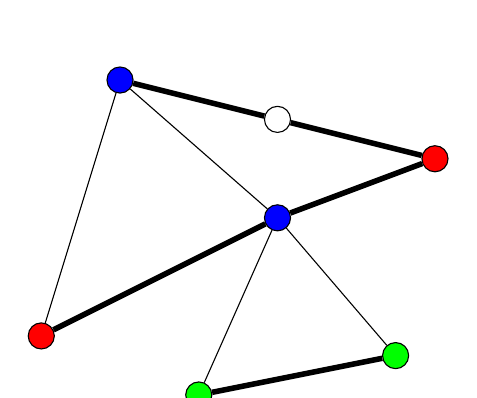
\begin{tikzpicture}[node distance={30mm}, main/.style = {draw, circle}] 
        \node[main, fill=blue] (1) at (4, 2) {}; 
        \node[main] (2) at (6, 1.5) {};
        \node[main, fill=red] (3) at (8, 1) {};
        \node[main, fill=blue] (4) at (6, 0.25) {};
        \node[main, fill=red] (5) at (3, -1.25) {};
        \node[main, fill=green] (6) at (5, -2) {};
        \node[main, fill=green] (7) at (7.5, -1.5) {};

        \draw [line width=2pt] (1) -- (2); \draw [line width=2pt] (2) -- (3);
        \draw [line width=2pt] (3) -- (4);
        \draw (1) -- (4); \draw (1) -- (5); 
        \draw [line width=2pt] (4) -- (5);
        \draw (4) -- (6); \draw (4) -- (7); \draw [line width=2pt] (6) -- (7);
    \end{tikzpicture} 
\end{center}\vspace{-0.25cm}
This problem can be formulated as a network design problem where the 
cut requirement function is
\[ f(S) = \begin{cases}
    1 & \text{if there exists $i = 1, \dots, k$ such that 
    $S \cap T_i \neq \varnothing$ and $S \cap T_i \neq T_i$}, \\
    0 & \text{otherwise.}
\end{cases} \] 
The fact that $f : 2^V \to \{0, 1\}$ is a proper function can be shown 
similarly to above.

\subsection{LP Formulation of the Network Design Problem} \label{subsec:7.2}
From now on, we assume that the cut requirement function 
$f : 2^V \to \{0, 1\}$ is proper. How do we solve network design problems 
under this assumption? This problem is $\NP$-hard in general 
since the Steiner tree problem is a special case of it. 
But we have nice approximation algorithms by way of linear programming. 

First, for ease of notation, we'll denote $\mathcal{K} = \{S \subseteq V : 
f(S) = 1\}$. Then the LP formulation of the network design problem, 
namely our primal LP (P), can be stated as follows. 
\begin{align*}
    \min\quad & \sum_{e\in E} c_e x_e \\ 
    \text{subject to}\quad & \sum_{e\in \delta(S)} x_e \geq 1 
    \quad \text{for all $S \in \mathcal{K}$} \\
    & x \geq \mathbf 0.
\end{align*}
Then the dual LP of (P), say (D), is given as follows.
\begin{align*}
    \max\quad & \sum_{S\in\mathcal{K}} 1 \cdot y_S \\ 
    \text{subject to}\quad & \sum_{S\in\mathcal{K}\,:\,e \in \delta(S)} y_S \leq c_e 
    \quad \text{for all $e\in E$} \\
    & y \geq \mathbf 0.
\end{align*}

\subsection{Iterative Rounding Approach} \label{subsec:7.3}
The iterative rounding approach for solving network design problems 
only makes use of the primal LP (P) above. The algorithm is
as follows: 
\begin{mdframed}[
    linewidth=1pt,
    linecolor=black,
    bottomline=false,topline=false,rightline=false,
    innerrightmargin=0pt,innertopmargin=0pt,innerbottommargin=0pt,
    innerleftmargin=1em,% Distance between vertical rule & proof content
    skipabove=0.75\baselineskip
]
{\bf Input.} A graph $G = (V, E)$, edge costs $c_e \geq 0$ for 
all $e \in E$, and a cut requirement function $f : 2^V \to \{0, 1\}$. 

{\bf Output.} A set of edges $F \subseteq E$ with value close to the optimum.
\begin{enumerate}[leftmargin=1.75cm, label={Step \arabic*.}]
    \item [{Step 0.}] Initialize $F \gets \varnothing$.
    \item Find an extreme optimal solution $\bar{x}$ for the primal LP
    (which can be done in polynomial time).

    \item Find $e' \in E$ such that $\bar{x}_{e'} = 0$ or $\bar{x}_{e'} \geq 1/2$.
    The existence of such an edge for $\bar{x}$ is guaranteed to 
    exist in the case where $f : 2^V \to \{0, 1\}$ is a proper function.

    \item If $\bar{x}_{e'} = 0$, then construct $G' = (V, E \setminus \{e\})$
    and keep the same costs for the remaining edges. 
    If $\bar{x}_{e'} \geq 1/2$, construct $G'$ from $G$ by contracting the 
    edge $e'$ and include $e'$ into $F$. 

    \item Recursively call the algorithm on $G'$ to obtain a solution $F'$. 
    Output $F \gets F' \cup F$. 
\end{enumerate}
\end{mdframed}\vspace{-0.25cm}
Note that the optimal value $\text{OPT}_{\text{primal IP}}$ for the network 
design problem is the optimal value of the primal LP (P) with added 
integrality constraints. By solving the primal LP, we only obtain 
the value $\text{OPT}_{\text{primal LP}}$, which gives us a lower
bound on the desired value via
\[ \text{OPT}_{\text{primal LP}} \leq \text{OPT}_{\text{primal IP}} \] 
since this is a minimization problem and any feasible solution to the IP is 
also feasible for the LP. It turns out that the iterative rounding 
approach produces a solution of cost at most $2 \cdot \text{OPT}_{\text{primal LP}}$
and hence at most $2 \cdot \text{OPT}_{\text{primal IP}}$. In particular, 
the iterative rounding approach is a $2$-approximation algorithm for the 
network design problem.

We won't prove that an edge $e' \in E$ such that $\bar{x}_{e'} = 0$ 
or $\bar{x}_{e'} \geq 1/2$ always exists when $f : 2^V \to \{0, 1\}$ is a 
proper function, as this is quite difficult. For the analysis, we'll assume 
this fact and show that the solution obtained of the algorithm is within a 
factor of $2$ of the optimum. This can be proven by induction on the number 
of edges $|E|$. 

{\bf Case 1.} Suppose that $\bar{x}_{e'} = 0$. Then the solution 
$x^*_e := \bar{x}_e$ for all $e \in E \setminus \{e'\}$ is still feasible 
for the LP constructed for $G' = (V, E \setminus \{e'\})$. By 
induction, we have that 
\[ c(F') \leq 2 \cdot \text{OPT}_{\text{primal LP for $G'$}} \leq 
2 \cdot \sum_{e \in E} c_e \bar{x}_e \leq 2 \cdot \text{OPT}_{\text{primal LP}}, \] 
where $F'$ is the output of the algorithm for $G'$.

{\bf Case 2.} Suppose that $\bar{x}_{e'} \geq 1/2$. Then the solution 
$x_e^* := \bar{x}_e$ for all $e \in E \setminus \{e'\}$ is still feasible 
for the LP constructed for $G'$ obtained by contracting $e'$ in $G$. 
By induction, we have that 
\[ c(F') \leq 2 \cdot \text{OPT}_{\text{primal LP for $G'$}} \leq 
2 \cdot \sum_{e \in E \setminus \{e'\}} c_e \bar{x}_e, \]
where $F'$ is the output of the algorithm for $G'$. Afterwards, we output 
$F' \cup \{e'\}$ for $G$, and we see that 
\[ c(F' \cup \{e'\}) \leq 2 \cdot \sum_{e \in E \setminus \{e'\}} c_e \bar{x}_E
+ c'_e \leq 2 \cdot \sum_{e \in E} c_e \bar{x}_e \] 
since $c_{e'} \leq 2c_{e'} \bar{x}_{e'}$ by the choice of $e'$, as desired. 

\subsection{Primal-Dual Approach} \label{subsec:7.4}
We now give another approximation algorithm for solving the network 
design problem, this time making use of the dual LP. The idea is to 
construct a feasible solution $y$ for the dual LP; based on this 
dual solution $y$, we construct the output $F \subseteq E$. Suppose we 
could argue that 
\[ c(F) \leq \alpha \cdot \sum_{S \in \mathcal{K}} y_S \] 
where $\sum_{S \in \mathcal{K}} y_S$ is the value of the dual solution $y$ 
and $\alpha \geq 1$ is some constant. We see that 
\[ \sum_{S\in\mathcal{K}} y_S \leq \text{OPT}_{\text{primal LP}} \leq 
\text{OPT}_{\text{primal IP}} \] 
where the first inequality is due to weak duality. This gives rise to an
$\alpha$-approximation algorithm.

The primal-dual approach is based on the notion of continuous growth. 
Over a time period, we pick some values $y_S$ where $S \in \mathcal{K}$
and increase them at the same rate, while the other values are kept fixed. 
\begin{enumerate}[(1)]
    \item At a time period, how do we select the subsets $S \in \mathcal{K}$ 
    for which to increase the values $y_S$?
    \item When do we stop increasing the values for the currently 
    selected sets $S \in \mathcal{K}$?
\end{enumerate}
To answer the first question, we will pick all the inclusion-wise minimal sets 
$S \in {\cal K}$ such that $\delta(S) \cap F = \varnothing$. In other words, 
these are the sets $S \subseteq V$ such that $f(S) = 1$ and $\delta(S) \cap F 
= \varnothing$, with the property that any proper subset $S' \subsetneq S$ will have 
$f(S') = 0$ or $\delta(S') \cap F \neq \varnothing$. 

Let $\mathcal{B} := \{S \in \mathcal{K} : \delta(S) \cap F = \varnothing\}$. 
We call $\mathcal{B}$ the collection of violated sets. Let
$\mathcal{D}$ be collection of minimal sets in $\mathcal{B}$. The following 
lemma tells us that $\mathcal{D}$ can be efficiently computed. 

\begin{lemma}{lemma:7.1} 
    For every $F \subseteq E$, we have that 
    \[ \mathcal{D} = \{S \subseteq V : \text{$S$ is a connected component of $(V, F)$ 
    such that $f(S) = 1$}\}. \]
\end{lemma}\vspace{-0.25cm}
\begin{pf}[Lemma~\ref{lemma:7.1}]
    $(\subseteq)$  Let $S_1, \dots, S_k$ denote the connected components of $(V, F)$, 
    and let $S \subseteq V$. If $S \cap S_i \neq \varnothing$ and 
    $S \cap S_i \neq S_i$, then we have $F \cap \delta(S) \neq \varnothing$. 
    In particular, for any $S \in \mathcal{B}$, we have that 
    \[ S = \bigcup_{j \in J} S_j \] 
    for some $J \subseteq \{1, \dots, k\}$. Since $f : 2^V \to \{0, 1\}$ 
    is a proper function, we have 
    \[ f(S) \leq \max_{j\in J} f(S_j). \] 
    Let $S \in \mathcal{D}$ so that $S$ is a minimal set in $\mathcal{B}$.
    By the above discussion, we can write $S = \bigcup_{j\in J} S_j$ for 
    some $J \subseteq \{1, \dots, k\}$. Since $f(S) = 1$, we see that 
    $f(S_j) = 1$ for some $j \in J$. Then $S_j$ is a connected component 
    of $(V, F)$, which implies that $\delta(S_j) \cap F = \varnothing$. 
    Therefore, $S_j$ is a violated set. Since $S$ is minimal, 
    it must be that $S = S_j$ for some $j = 1, \dots, k$, so $S$ 
    is a connected component of $(V, F)$. 

    $(\supseteq)$ Suppose that $S$ is a connected component of $(V, F)$. 
    Then $\delta(S) \cap F = \varnothing$, so $S$ is a violated set. 
    But for every nonempty proper subset $S' \subsetneq S$, we have 
    $\delta(S') \cap F \neq \varnothing$ because inside the connected 
    component, considering the cut induced by some proper subset of vertices 
    gives rise to an edge. This implies that $S$ must be minimal, so 
    we are done. \qed 
\end{pf}\vspace{-0.25cm}

As a consequence, we obtain the following corollary. 

\begin{cor}{cor:7.2}
    A subset $F \subseteq E$ is a feasible solution to the network design 
    problem if and only if for every component $S$ of $(V, F)$, 
    we have $f(S) = 0$. 
\end{cor}\vspace{-0.25cm}

Now, let's consider the question of when to stop increasing the values of $y_S$. 
As stated before, we will increase the values of $y_S$ for all $S \in \mathcal{D}$
at the same rate, and leave $y_S$ for $S \notin \mathcal{D}$ unchanged. 
We do this until there is an edge $e \in E$ such that $e \in \delta(S)$ 
for some $S \in \mathcal{D}$ and 
\[ \sum_{S\in\mathcal{K}\,:\,e\in\delta(S)} y_S = c_e. \] 
That is, the corresponding constraint for $e \in E$ in the dual LP becomes tight. 
In this case, we call the edge $e$ {\bf tight}. Once we stop, we will 
include all the tight edges into $F$. 

Putting everything together, the primal-dual approach to solve network 
design problems is as follows.

\begin{mdframed}[
    linewidth=1pt,
    linecolor=black,
    bottomline=false,topline=false,rightline=false,
    innerrightmargin=0pt,innertopmargin=0pt,innerbottommargin=0pt,
    innerleftmargin=1em,% Distance between vertical rule & proof content
    skipabove=0.75\baselineskip
]
{\bf Input.} A graph $G = (V, E)$, edge costs $c_e \geq 0$ for 
all $e \in E$, and a cut requirement function $f : 2^V \to \{0, 1\}$. 

{\bf Output.} A set of edges $F \subseteq E$ with value close to the optimum.
\begin{enumerate}[leftmargin=1.75cm, label={Step \arabic*.}]
    \item Let $F = \varnothing$ and let $y_S = 0$ for all $S \in \mathcal{K}$.
    Let $\mathcal{D}$ be the collection of minimal violated sets with respect 
    to $F$. (At this stage, these are the isolated vertices.)

    \item While $\mathcal{D} \neq \varnothing$:
    \begin{enumerate}[label={Step 2.\arabic*.}]
        \item Increase $y_S$ for $S \in \mathcal{D}$ at the same rate 
        until some edge $e \in E$ becomes tight.
        \item Update $F := F \cup T$ where $T$ is the set of all tight edges. 
        Update $\mathcal{D}$ with respect to this new $F$. 
    \end{enumerate}

    \item {\bf (Reverse delete.)} Let $F = \{e_1, \dots, e_k\}$ where the 
    index corresponds to the order that the edges were inserted to $F$. 
    Iterate backwards through the list; that is, start from $i = k$ 
    and go down to $i = 1$. For each $i$, if $F \setminus \{e_i\}$ is feasible 
    for the network design problem, update $F := F \setminus \{e_i\}$.
\end{enumerate}
\end{mdframed}\vspace{-0.25cm}

\newpage

\end{document}
